\documentclass[answers, a4paper, 11pt]{exam}
\usepackage{amsmath}
\usepackage{amssymb}
\usepackage{amsthm}
\usepackage[italian]{babel}
\usepackage{ccicons}
\usepackage{hyperref} % Has to be loaded before cleveref
\usepackage{cleveref}
\usepackage[utf8]{inputenc} % Has to be loaded before csquotes
\usepackage[autostyle=false, style=english]{csquotes}
\usepackage[margin=2cm]{geometry}
\usepackage{graphicx}
\usepackage{mathrsfs}
\usepackage{multicol}
\usepackage{relsize}
\usepackage{parskip}
\pagestyle{plain}
\graphicspath{{./images/}}
\MakeOuterQuote{"}
\setlength{\columnseprule}{.4pt}
\renewcommand{\solutiontitle}{\noindent\textbf{R:}\enspace}
\newcommand{\concat}{\#\#}
\def\dbar{{\mathchar'26\mkern-12mu d}}
\title{Sicurezza dell'Informazione M}
\author{Kevin Michael Frick}
\begin{document}
\maketitle
\textbf{Titoli di testa}: Ringrazio di cuore Corinna e Giacomo per l’aiuto nella stesura di questo documento, nella preparazione di questo esame e soprattutto nella conservazione, pur stentata, della sanit`a mentale. Vi si vuole bene ragazz*.
\begin{questions}
\question \textbf{Meccanismi crittografici di base}
\begin{parts}
\part Si enuncino le proprietà delle funzioni hash crittograficamente sicure.
\begin{solution}
Una funzione hash crittografica $H(x)$ in generale deve presentare quattro proprietà:
\begin{enumerate}
\item Efficienza: il calcolo di $H(x)$ è computazionalmente facile $\forall x$.
\item Robustezza debole alle collisioni: per ogni $x$ è computazionalmente infattibile trovare $y \neq x : H(y) = H(x)$.
	Per garantire resistenza debole bastano 160 bit di hash.
\item Resistenza forte alle collisioni: è infattibile trovare una qualunque coppia $y, x: y \neq x \land H(y) = H(x)$.
	Un esempio della differenza tra resistenza debole e forte si vede con il paradosso del compleanno: date 253  persone, la probabilità che, scelto un giorno, almeno una persona compia gli anni quel giorno è maggiore del 50\%.
		Invece, per avere una probabilità superiore al 50\% che due persone siano nate lo stesso giorno, qualunque esso sia, bastano 23 persone.
		Il numero di bit che garantisce la resistenza forte è circa il doppio di quelli necessari per garantire la resistenza debole, quindi 320 bit.
		Per sicurezza e completezza si usano 512 bit.
		Un attacco basato sul paradosso del compleanno consiste nel prendere un messaggio favorevole alla vittima e trasformarlo in un messaggio con lo stesso hash ma favorevole all'intrusore. L'intrusore genera quindi $2^{n/2}$ messaggi diversi dei quali calcola lo hash.
		Per il paradosso del compleanno, l'intrusore dovrebbe riuscire a trovare una coincidenza e riruscire quindi a inviare e far accettare il proprio messaggio invece di quello originario.
\item Unidirezionalità: il calcolo di $H^{-1}(h) \forall h : H(x) = h$ è infattibile.
L'unidirezionalità è particolarmente importante se la funzione hash viene utilizzata per autenticare un dato, ad esempio accodando a $m$ il suo hash quando concatenato a un segreto $s$.
\end{enumerate}
\end{solution}
\part Si descrivano le proprietà di Pseudo Random Number Generator, True RNG e PRNG sicuro. A cosa serve il seed?
\begin{solution}
	Una chiave di un cifrario deve essere generata in maniera casuale e imprevedibile.
	La proprietà di casualità richiede che ogni bit sia statisticamente indipendente dagli altri ed equiprobabile rispetto agli altri.
	Per verificare la proprietà di casualità si utilizza un insieme di test: si conta il numero di 1 e 0, si divide la sequenza in sottosequenze e si controlla che siano diverse tra loro, si contano i Run e i Long Run.
	\begin{itemize}
		\item Un TRNG è un generatore di numeri casuali che si serve di segnali provenienti da fenomeni fisici, ad esempio registrati da un microfono o da altre periferiche del calcolatore.
Questi segnali vengono registrati digitalizzati ed  elaborati (deskewing) prima di venire memorizzati.
I TRNG possono produrre dati casuali a frequenza relativamente bassa.
	Inoltre, i TRNG non garantiscono la riproducibilità esatta, ovvero non hanno la possibilità di generare sequenze di numeri casuali identici come è richiesto da alcuni tipi di algoritmi.
\item Un PRNG è un generatore di numeri casuali che si serve di una macchina a stati finiti basata su algoritmi deterministici che generano sequenze di numeri a partire da un dato iniziale detto \textit{seed}.
Un PRNG può produrre dati a frequenza molto alta e permette di riprodurre le sequenze utilizzando lo stesso seed, ma ciò significa che in assenza di accorgimenti appositi può essere possibile prevedere i numeri generati successivamente partendo da una sequenza di numeri già generati.
Inoltre, le sequenze generate da un PRNG sono finite e destinate a presentare ripetizioni, presentano cioè un periodo di funzionamento e non garantiscono l'imprevedibilità.
Un esemoio di PRNG deterministico è il generatore lineare congruenziale.
\item Un PRNG sicuro (Cryptographically Secure PRNG) garantisce la proprietà di imprevedibilità: deve essere computazionalmente molto difficile risalire al seed o ai numeri generati in futuro partendo da una sequenza di numeri generati.
	Ciò implica che il periodo di ripetizione (ovvero la lunghezza delle sequenze possibili) sia molto grande ($>10^{50}$), che il seed sia imprevedibile (possibilmente generato da un TRNG) e che dati $L(\cdot)$ bit di una sequenza generata non sia possibile prevedere l'$L+1$-esimo bit con probabilità maggiore di 0.5 (\textit{next-bit test}).
Ricordando che un PRNG, essendo una macchina a stati finiti, presenta una funzione di stato futuro e una di uscita, l'imprevedibilità richieda che una di queste due funzioni siano unidirezionali.
Esempi di PRNG sicuri sono il \texttt{SecureRandom} di Java, la cifratura di un contatore utilizzando il seed come chiave e il PRNG X9.17.
	\end{itemize}
	Un buon RNG è ottenuto usando un TRNG per generare il seed e poi usare un PRNG con un periodo di funzionamento molto lungo in cui almeno una delle due funzioni (stato futuro o uscita) unidirezionale.
\end{solution}
\part Si descriva l'attacco con estensione delle funzioni hash crittograficamente sicure servendosi di opportuni schemi.
\begin{solution}
Gli algoritmi di hash crittograficamente sicuri si basano sul principio della compressione iterata.
Per calcolare uno hash ci si serve di una funzione di compressione $f$ resistente alle collisioni e facile da calcolare, che abbia come stato interno un dato di $n$ bit e come input uno di $r$ bit, $r > n$ e produca una stringa di $n$ bit.
Si suddivide il messaggio $m$ da comprimere in blocchi di lunghezza $r$ e si applica la funzione di compressione a ogni blocco, assumendo come stato interno il risultato della compressione precedente, $h_i = f(m{i - 1}, h_{i - 1})$.
Lo stato iniziale $h_0$ è detto vettore di inizializzazione, il risultato finale $h$ è l'\textit{impronta
} $H(m)$.
L'attacco con estensione è una vulnerabilità del protocollo di comunicazione che prevede che con ogni messaggio $m$ venga inviato al destinatario un "autenticatore" $H(s\concat m)$, con $s$ segreto concordato, nel caso in cui alla fine di $m$ non venga aggiunta un'indicazione di quanto è lungo.
Un attaccante, dopo aver intercettato $m$ e $H(s\concat m)$,  può individuare un'estensione $m'$ e formare un messaggio $m\concat m'$, calcolando $H(m')$ fornendo come stato iniziale non $h_0$ ma $H(s\concat m)$ intercettato.
Il risultato ottenuto, per costruzione, è uguale a quella di $H(s\concat(m\concat m'))$ e il messaggio viene giudicato valido.
Per cercare di prevenire l'attacco di estensione si aggiunge un padding nel blocco finale che contiene la lunghezza del messaggio.
Ciò diminuisce la probabilità di essere vulnerabili a questo attacco ma non lo risolve.
Di seguito viene riportato lo schema dell'attacco di length extension.

\includegraphics[width=0.6\textwidth]{lengthext}

\end{solution}
\part Si descriva la differenza tra identificazione passiva e attiva.
\begin{solution}
	\begin{itemize}
		\item L'identificazione passiva avviene mediante l'uso di un identificativo e una password.
Nella sua forma più semplice, l'utente trasmette in chiaro ID e password, la macchina atta all'identificazione estrae da un database la password corrispondente all'ID e la confronta con quella fornita.
Se coincidono, l'utente è identificato.
\item L'identificazione attiva prevede una prova di identità che cambi continuamente.
È possibile sviluppare un protocollo di identificazione attiva mediante una \textit{password usa e getta}, una \textit{sfida e risposta} o una \textit{prova d'identità a conoscenza zero}.
In generale, un protocollo di identificazione attiva richiede di impostare un calcolo di una prova d'identità che deve essere facile per chi conosce un'informazione segreta e difficile per chi non la conosce, anche se dispone di prove inviate in precedenza.
Un esempio di identificazione attiva è usata nella tecnologia GSM: un'entità mobile si deve identificare presso una BTStation, la quale però non può identificare ogni entità mobile istantaneamente perché non ne può avere conoscenza.
Delega uindi lo Home Location Registry, che tiene traccia di tutte le entità mobili disponibili e memorizza un segreto per ciascuna SIM.
Il protocllo prevede che l'entità mobile invii l'identificativo a BTS, il quale lo inoltra a HLR< che a sua volta genera una sfida $R$ e la inoltra a BTS, che la rigira all'entità mobile.
Sia l'entita che HLR producono $H(s \concat R)$, la inoltrano a BTS il quale confronta i due termini.
Se l'esito è positivo, l'entità è legittima.
	\end{itemize}
\end{solution}
\end{parts}
\question \textbf{Cifrari simmetrici e meccanismi simmetrici per la riservatezza e l'autenticazione. Fondamenti di teoria dei numeri. Scambio DH. }
\begin{parts}
\part Si evidenzi la differenza tra cifratura monoalfabetica e polialfabetica.
\begin{solution}
	\begin{itemize}
		\item La cifratura monoalfabetica sostituisce a uno o più simboli nel testo in chiaro uno e un solo simbolo nel testo cifrato proveniente dallo stesso alfabeto in cui e scritto il testo in chiaro.
	Si hanno quindi $26! = 4 \cdot 10^{26}$ possibili alfabeti, ma uno spazio delle chiavi così grande non serve a nulla.
Il punto debole della sostituzione monoalfabetica è la vulnerabilità ad attacchi di tipo statistico: conoscendo le ridondanze del linguaggio naturale in cui è scritto il messaggio in chiaro (e.g. la lettera E è la più comune nelle parole inglesi) è possibile cercare queste ridondanze anche nel testo cifrato e servirsene per rompere la cifratura.
È importante quindi mascherare la ridondanza, creando un cifrario con trasposizione e sostituzione nel quale tutti i caratteri cifrati siano quasi equiprobabili, in modo da rendere molto difficile la decifratura.
\item La cifratura polialfabetica si avvale di più alfabeti per poter scegliere tra più omofoni il simbolo che sarà inserito nel testo cifrato secondo una funzione della posizione del simbolo all'interno della stringa.
Il punto debole della sostituzione polialfabetica è che, data una chiave lunga $l$, simboli distanti $l$ l'uno dall'altro nel testo cifrato discendono dalla stessa sostituzione alfabetica.
	\end{itemize}
\end{solution}
\part Si elenchino i cifrari simmetrici che permettono la decifratura in parallelo.
	\begin{solution}
		Dato che ECB prevede che non ci siano dipendenze tra i blocchi di testo da cifrare o tra quelli cifrati, è possibile parallelizzare sia la decifratura che la cifratura.
		Se ci si serve di CBC, invece è possibile parallelizzare solo la decifratura se si hanno a disposizione tutti i blocchi di testo cifrato.
		Usando la cifratura CTR si opera come in ECB ma aggiungendo un'operazione di XOR con il cifrato di un contatore.
		È quindi possibile decifrare in parallelo senza problemi.
	\end{solution}
	\part Si descriva il problema della malleabilità dei cifrari simmetrici a flusso.
	\begin{solution}
		La malleabilità è un attacco attivo che consiste nello sfruttare la proprietà dello XOR secondo cui $a \oplus b \oplus a = b$ per far decifrare un  messaggio arbitrario al destinatario.
		Siano $m$ un messaggio, $k$ flusso di chiavi, $p$ un messaggio di un malintenzionato.
		Un malintenzionato intercetta il messaggio $a \oplus k$ e trasmette al destinatario $a \oplus k \oplus p$; in questo modo, il destinatario leggerà $a \oplus p$ invece di $a$.
		In generale, se l'intrusore conosce il formato di $m$, fare ricevere il messaggio $m'$ sfruttando la malleabilità richiede di trovare $p$ tale che $m \oplus p = m'$.
	\end{solution}
\part Si descrivano i cifrari simmetrici a flusso, autosincronizzanti e a flusso sincrono. Perché non è possibile usare un TRNG in cifrari a flusso?
In quali casi un cifrario a flusso sincrono perde sincronismo?
Quali sono le condizioni necessarie per rendere sicuro l'utilizzo di un cifrario a flusso sincrono?
\begin{solution}
	Un cifrario è simmetrico se sorgente e destinazione condividono la stessa chiave, usata sia per cifrare che per decifrare.

		I cifrari simmetrici a flusso si richiamano al funzionamento dello \textit{one-time pad}.
	Essi trasformano un bit alla volta eseguendo lo XOR tra il bit da cifrare e un bit aleatorio che viene genrato tramite un PRNG sicuro partendo da un seed imprevedibile.
	I cifrari simmetrici vengono usati per comunicazioni orientate al flusso (audio, GSM, video web ecc.).
	I cifrari a flusso necessitano di \textit{sincronismo}, altrimenti la decifrazione non avviene correttamente; un cifrario a flusso è \textit{sincrono} se il bit di testo cifrato dipende solo dal bit aleatorio generato dal PRNG e dal bit in chiaro, e \textit{autosincronizzante} se il bit cifrato viene influenzato dai bit aleatori precedentemente generati, memorizzati in un registro a scorrimento.

Un cifrario a flusso sincrono perde sincronismo in caso di inserimento o cancellazione di un bit.
Nel caso di cifrari a flusso sincrono la perdita di sincronismo è permanente, mentre nel caso dei cifrari autosincronizzanti la perdita è transitoria e il flusso si regolarizza appena il bit errato esce dal registro a scorrimento.

Perché un cifrario a flusso sincrono sia sicuro è necessario che la funzione interessata dalla casualità (avanzamento di stato o generazione dell'output) sia unidirezionale, in modo che non sia possibile risalire alla chiave da un messaggio cifrato, che il PRNG usato sia sicuro e che la chiave venga usata una sola volta.
Non è possibile usare un TRNG in cifrari a flusso perché il RNG viene usato per generare la chiave, che deve essere a conoscenza della sorgente e del destinatario.
\end{solution}
\part Si descriva il funzionamento di Electronic Code Book (ECB) e Cipher Block Chaining (CBC) e i vantaggi e gli svantaggi di ognuno dei due.
Si discuta l'importanza della pseudocasualità dell'$IV$ per CBC. Se, in una comunicazione cifrata con CBC, il destinatario perde il valore di IV, è possibile recuperare il messaggio?
\begin{solution}
	\begin{itemize}
		\item 	I cifrari a blocchi si richiamano al funzionamento del cifrario di Playfair.
	Essi trasformano un insieme numeroso di bit (detto blocco) alla volta secondo una regola fissa determinata da una chiave di lunghezza fissa.
	Un cifrario a blocchi non è sempre più sicuro di un cifrario a flusso; la sicurezza dipende dall'uso che ne viene fatto, in particolare dalla scelta della chiave.
Il cifrario a blocchi ECB suddivide il testo $m$ in $n$ blocchi $m_i, i \in 1..n$ e cifra ciascun blocco con una funzione $E_k$ e una chiave $k$, uguali per tutti i blocchi.
Nel caso in cui l'ultimo blocco sia più corto degli altri, vengono aggiunti dei bit in eccesso (padding).
La regola di trasformazione $E_k$ è una sostituzione monoalfabetica.
ECB permette di parallelizzare la cifratura (cifrando più blocchi alla volta) e garantisce la non propagazione degli errori fuori dal blocco interessato.
Tuttavia, presenta un alto grado di determinismo: a blocchi identici in chiaro corrispondono blocchi identici cifrati.
\item CBC prevede che ogni blocco del testo in chiaro sia sommato modulo 2 con il blocco cifrato precedente, poi cifrato a sua volta.
Il primo blocco è sommato con un valore casuale $IV$ per impedire a un eventuale intruso di dedurre che due messaggi abbiano la stessa intestazione.
	Chiaramente $IV$ deve essere conosciuto da entrambe le parti: può essere inviato come primo blocco del cifrato oppure concordato in partenza.
In ogni caso, $IV$ dev'essere pseudocasuale (per poter essere conosciuto da entrambe le parti), imprevedibile e usato una sola volta (per assicurare non determinismo).
Lo standard WEP è un protocollo per creare seed sempre diversi per permettere la generazione di un flusso di chiavi sempre diverso.
WEP prevede che IV e la chiave vengano usati per generare il seed, da dare come argomento al PRNG che genererà il flusso di chiave da mettere in XOR con il testo cifrato.
	IV è lungo 24 bit, quindi dopo $2^{24}$ generazioni il seed si ripeterà, rendendo WEP vulnerabile all'attacco two-time keys, una tipologia di attacco comunque passiva.
	Ogni cifrario simmetrico utilizzato per la riservatezza può comunque essere sempre attaccato tramite un attacco attivo.
	CBC risolve il problema del determinismo, ma fa perdere la possibilità di parallelizzare la cifratura, soffre di propagazione degli errori e non garantisce alcun tipo di verifica di integrità.
	\end{itemize}

Di seguito viene riportato lo schema di implementazione di CBC.

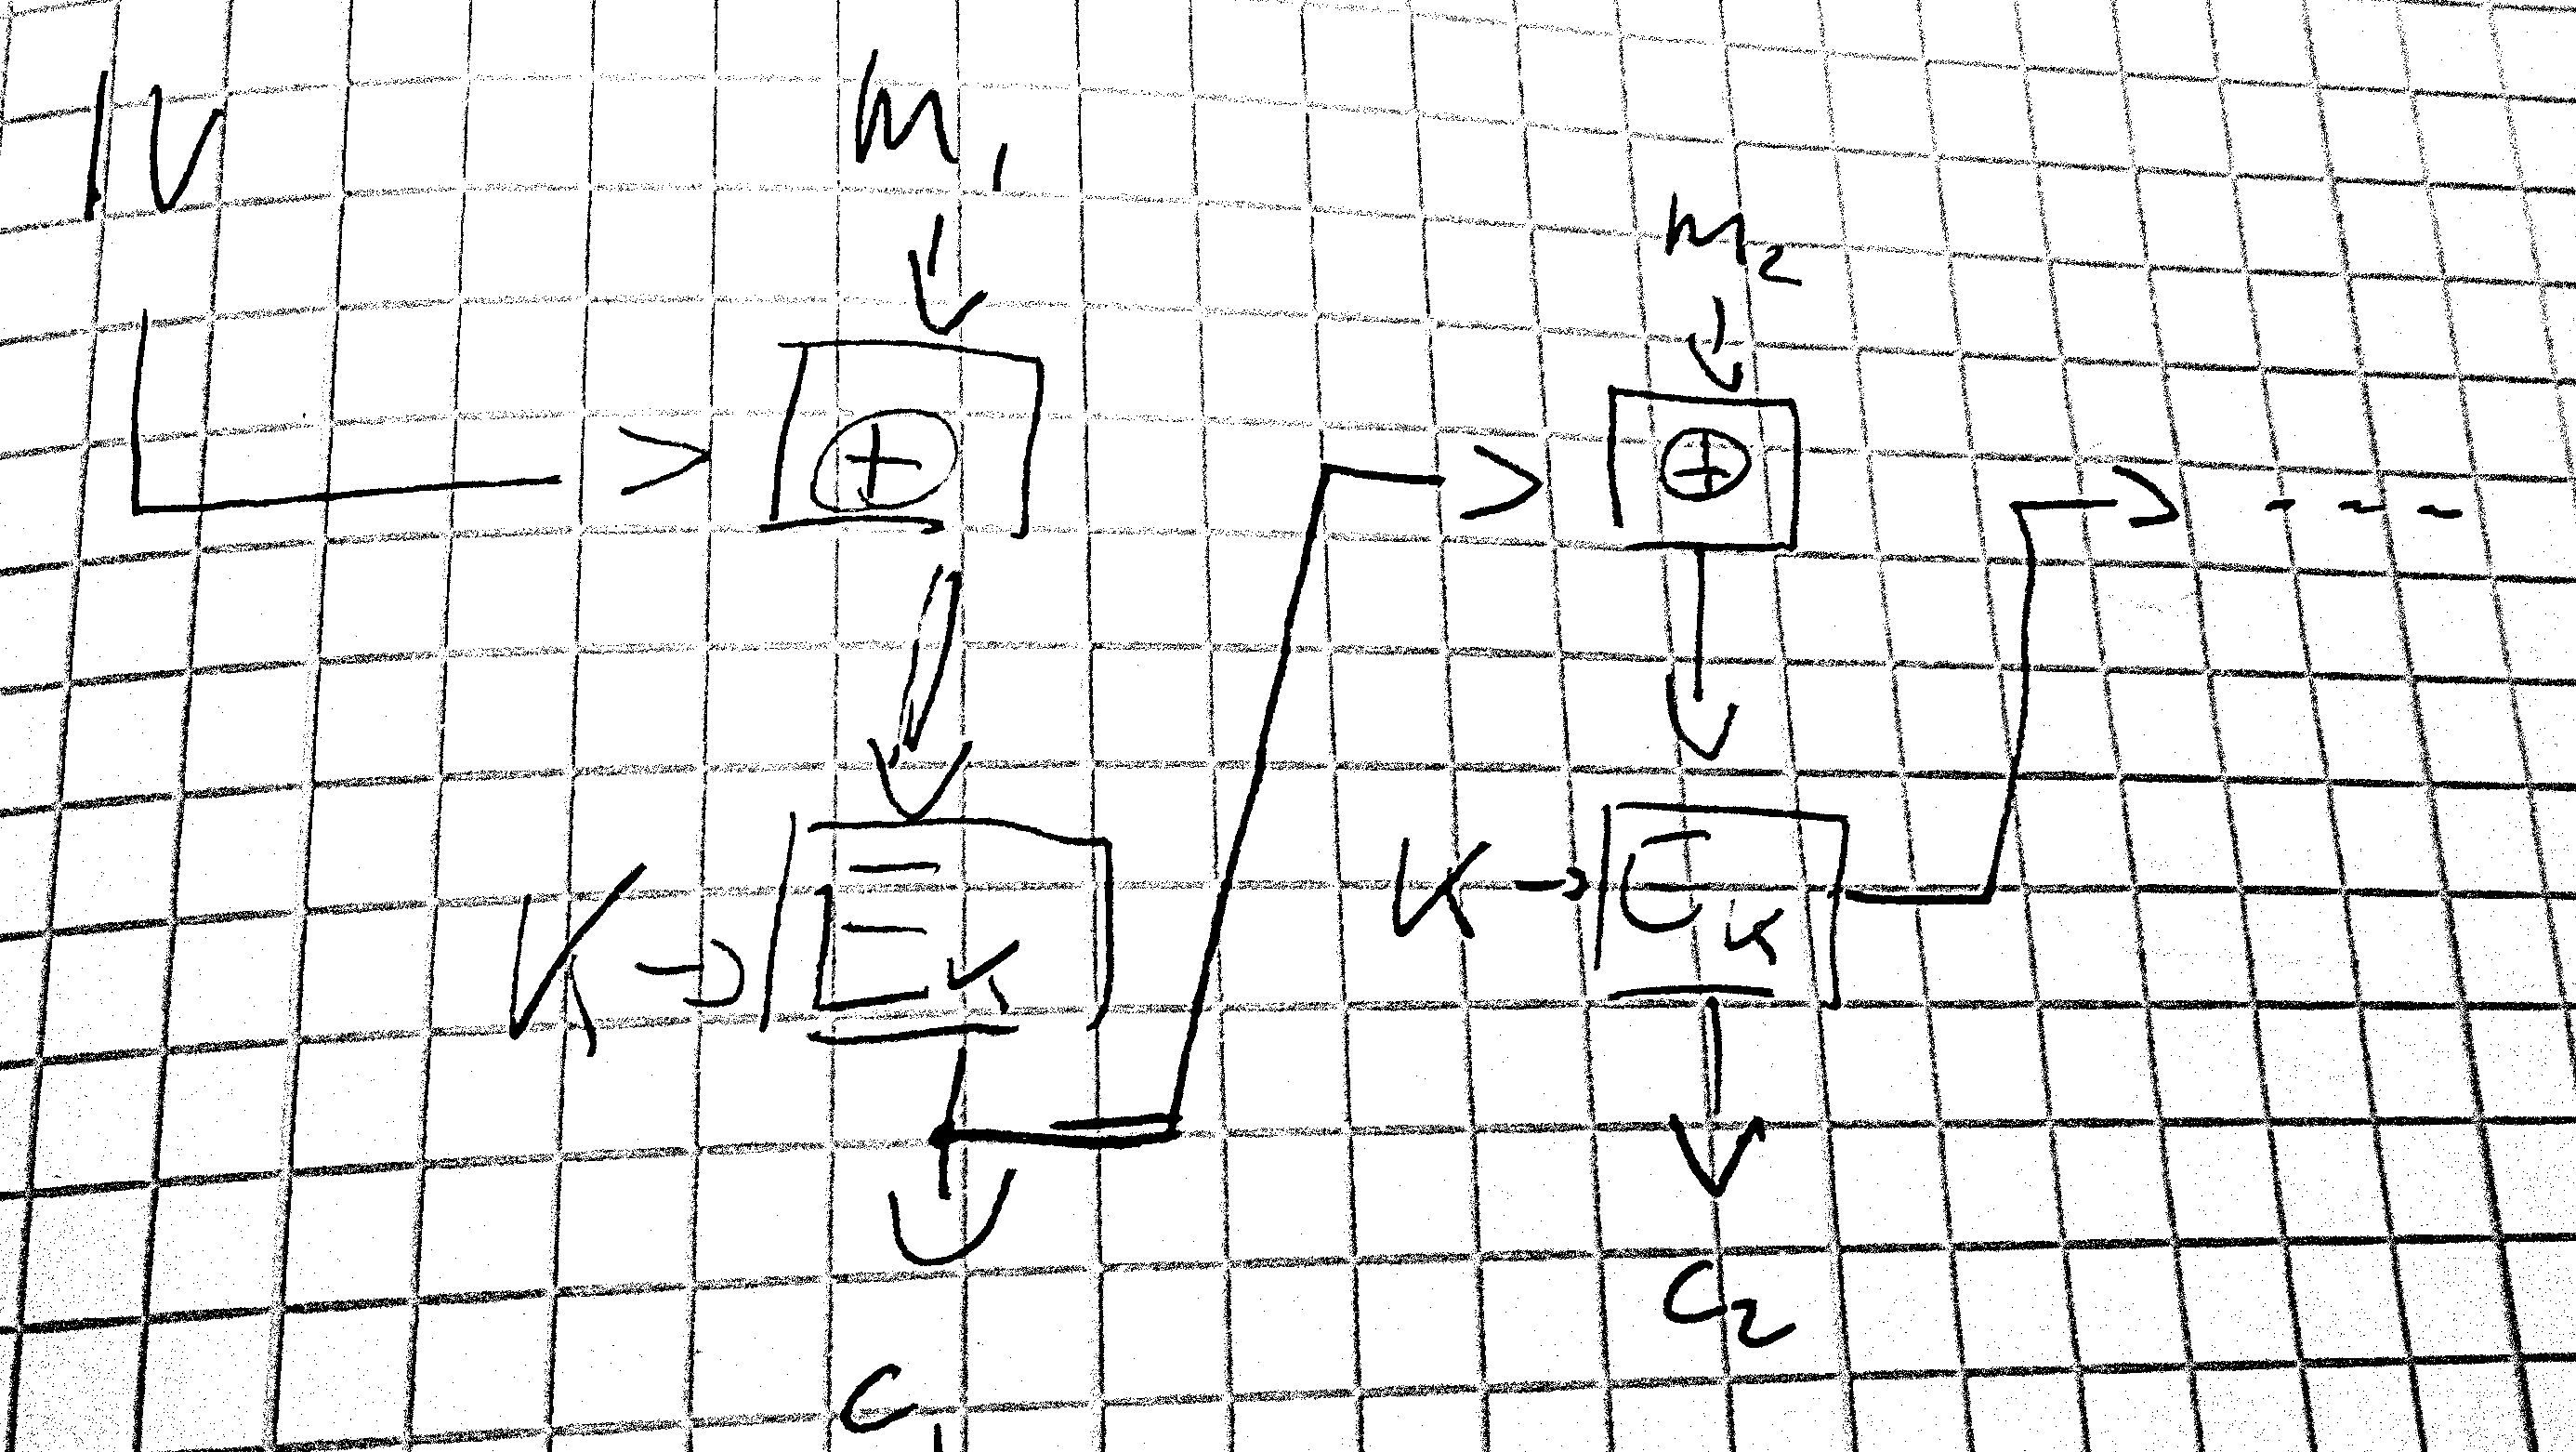
\includegraphics[width=0.6\textwidth]{cbc}

	È improbabile "dimenticarsi" di $IV$, dato che viene trasmesso in chiaro e contenuto nel primo blocco della comunicazione $C_0$.
	Anche nel caso in cui $C_0$ non sia $IV$ in chiaro, ma sia $C_0 = E_k(IV)$ avremmo comunque k per risalire a IV.
	Se per assurdo ci si scordasse di $IV$, la decifratura parte dall’ultimo blocco cifrato fino al primo, dunque senza $IV$ si può decifrare tutto tranne il primo blocco.
\end{solution}
\part In quali casi è più opportuno usare cifrature a blocchi o a flusso?
\begin{solution}
I cifrari a flusso sono tipicamente più veloci di quelli a blocco e richiedono meno memoria, dato che lavorano su pochi bit alla volta e non hanno "riporti" da blocchi precedenti.
I cifrari a blocco sono più suscettibili agli errori di trasmissione, mentre in un cifrario a flusso un errore su un bit non ha ripercussioni sugli altri bit.
I cifrari a flusso non garantiscono autenticazione o integrità, ma solo confidenzialità; alcuni tipi di cifrari a blocco, invece, possono garantire anche integrità.
Per questi motivi, i cifrari a flusso sono consigliabili quando la quantità di dati è sconosciuta o continua, come nelle trasmissioni su reti, mentre i cifrari a blocco lo sono quando è nota la quantità di dati da trasferire, come nel caso di file, protocolli a richiesta e risposta o campi dati prefissati.
\end{solution}
\part Si descrivano il modello di Feistel e il Data Encryption Standard (DES).
Su cosa si basa il blocco $F(\cdot)$ del modello di Feistel in DES?
\begin{solution}
Il modello di Feistel prevede che ogni blocco di testo cifrato sia ottenuto dal corrispondente blocco in chiaro iterando più volte una sostituzione e una trasposizione.
In generale, un blocco di testo $(L_i \concat R_i)$ lungo $2w$ bit è generato a partire da quello precedente seguendo le relazioni
\begin{equation}
\begin{array}{ll}
L_i &= R_{i-1} \\
R_i &= L_{i-1} \oplus F(R_{i-1}, k_i)
\end{array}
\label{eq:feistel}
\end{equation}
Ogni round si serve di una regola di sostituzione diversa, funzione della sottochiave $k_i$.
La decrittazione si esegue con lo stesso algoritmo, invertendo l'ordine delle $k_i$.
Prima della concatenazione che permette di ottenere il testo cifrato, $L_n$ e $R_n$ vengono nuovamente scambiati di posto.
Di seguito viene riportato uno schema del funzionamento del cifrario di Feistel.

\includegraphics[width=0.6\textwidth]{feistel}

Il DES è una implementazione di Feistel che usa 16 round, blocchi di 64 bit e una chiave di 64 bit di cui 8 di parità.
La $F(\cdot)$ di DES prevede in cascata una espansione e permutazione da 32 a 48 bit, una somma modulo 2 del risultato con la sottochiave, una sostituzione e scelta che fornisce un dato di 32 bit e una permutazione senza chiave.
\end{solution}
\part Si descriva il BEAST Attack.
\begin{solution}
	Il BEAST attack è un attacco attivo a SSL/TLS 1.0 quando è configurato per usare CBC con  un vettore di inizializzazione negoziato tra le parti prima dello scambio dei dati e prevedibile.
	Il BEAST attack è possibile in SSL/TLS 1.0 perché il messagggio è diviso in pacchetti IP che dovrebbero essere cifrati indipendentemente, mentre ciò non avviene:  un intrusore intercetta l'ultimo blocco di un pacchetto e sa che verrà usato come IV del pacchetto successivo.
	Un intrusore sa che i mesaggi sono strutturati, ha informazioni sulla struttura e vuole verificare una propria ipotesi sui contenuti del messaggio, ad esempio se ogni blocco contiene una parola e l'intrusore vuole verificare la seconda parola.
	Un esempio di BEAST attack è il seguente.
	Osservando il primo blocco di cifrato $C_1$ e il vettore di inizialzizazione $IV$  e potendo iniettare il successivo blocco di testo in chiaro $P_2$, l'intrusore può verificare se $P_1 = x$ iniettando $P_2 = x \oplus IV \oplus C_1$.
	Seguendo il procedimento di CBC, si ha $C_2 = E(P_2 \oplus C_1) = E(x \oplus IV \oplus C_1 \oplus C_1) = E(x \oplus IV)$, ma se $P_1 = x$ allora $C_2 = C_1$.
\end{solution}
\part Si descrivano gli schemi per verificare l'origine di un documento.
\begin{solution}
Per verificare l'origine di un messaggio è necessario che la sorgente apporti al documento una trasformazione $S(\cdot)$ che deve essere computazionalmente difficile eseguire per qualunque altra parte.
È possibile garantire l'autenticità tramite firma digitale o hash del messaggio e di un segreto.
L'invio di uno hash del messaggio e del segreto non garantisce il non ripudio perché entrambe le parti devono conoscere il segreto $s$.
Di seguito sono riportati gli schemi per i due casi.

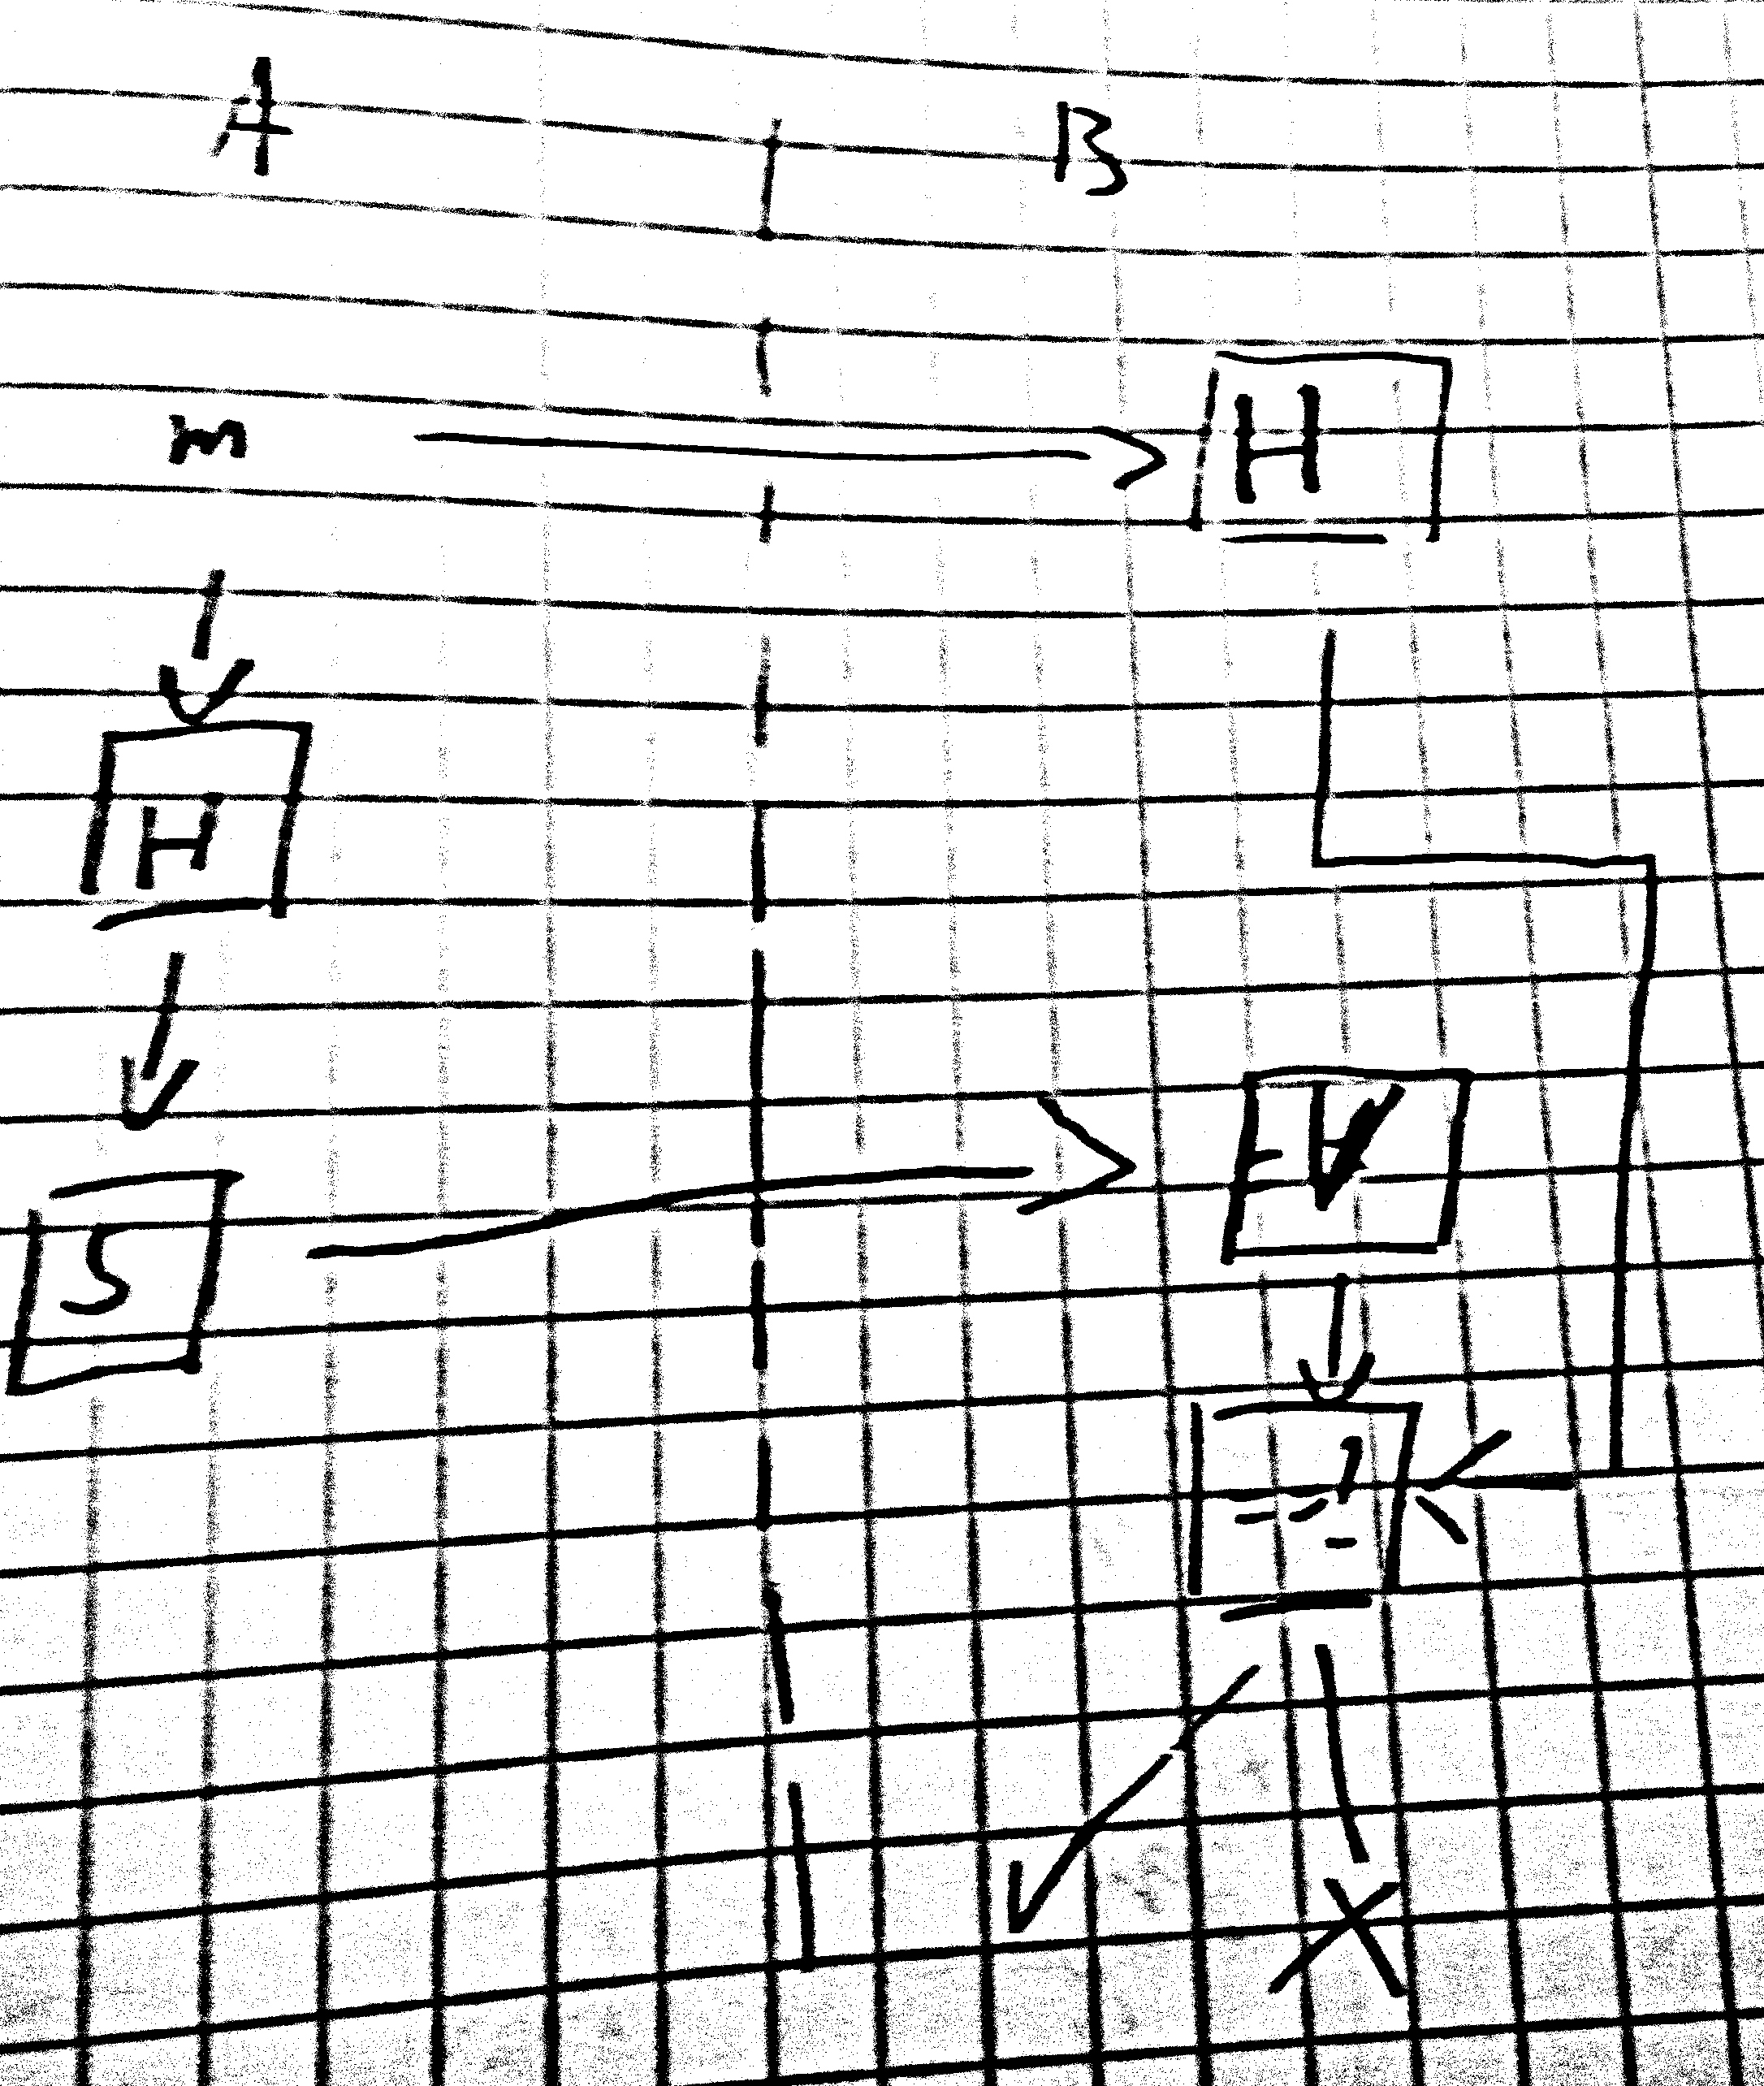
\includegraphics[width=0.6\textwidth]{authsign}


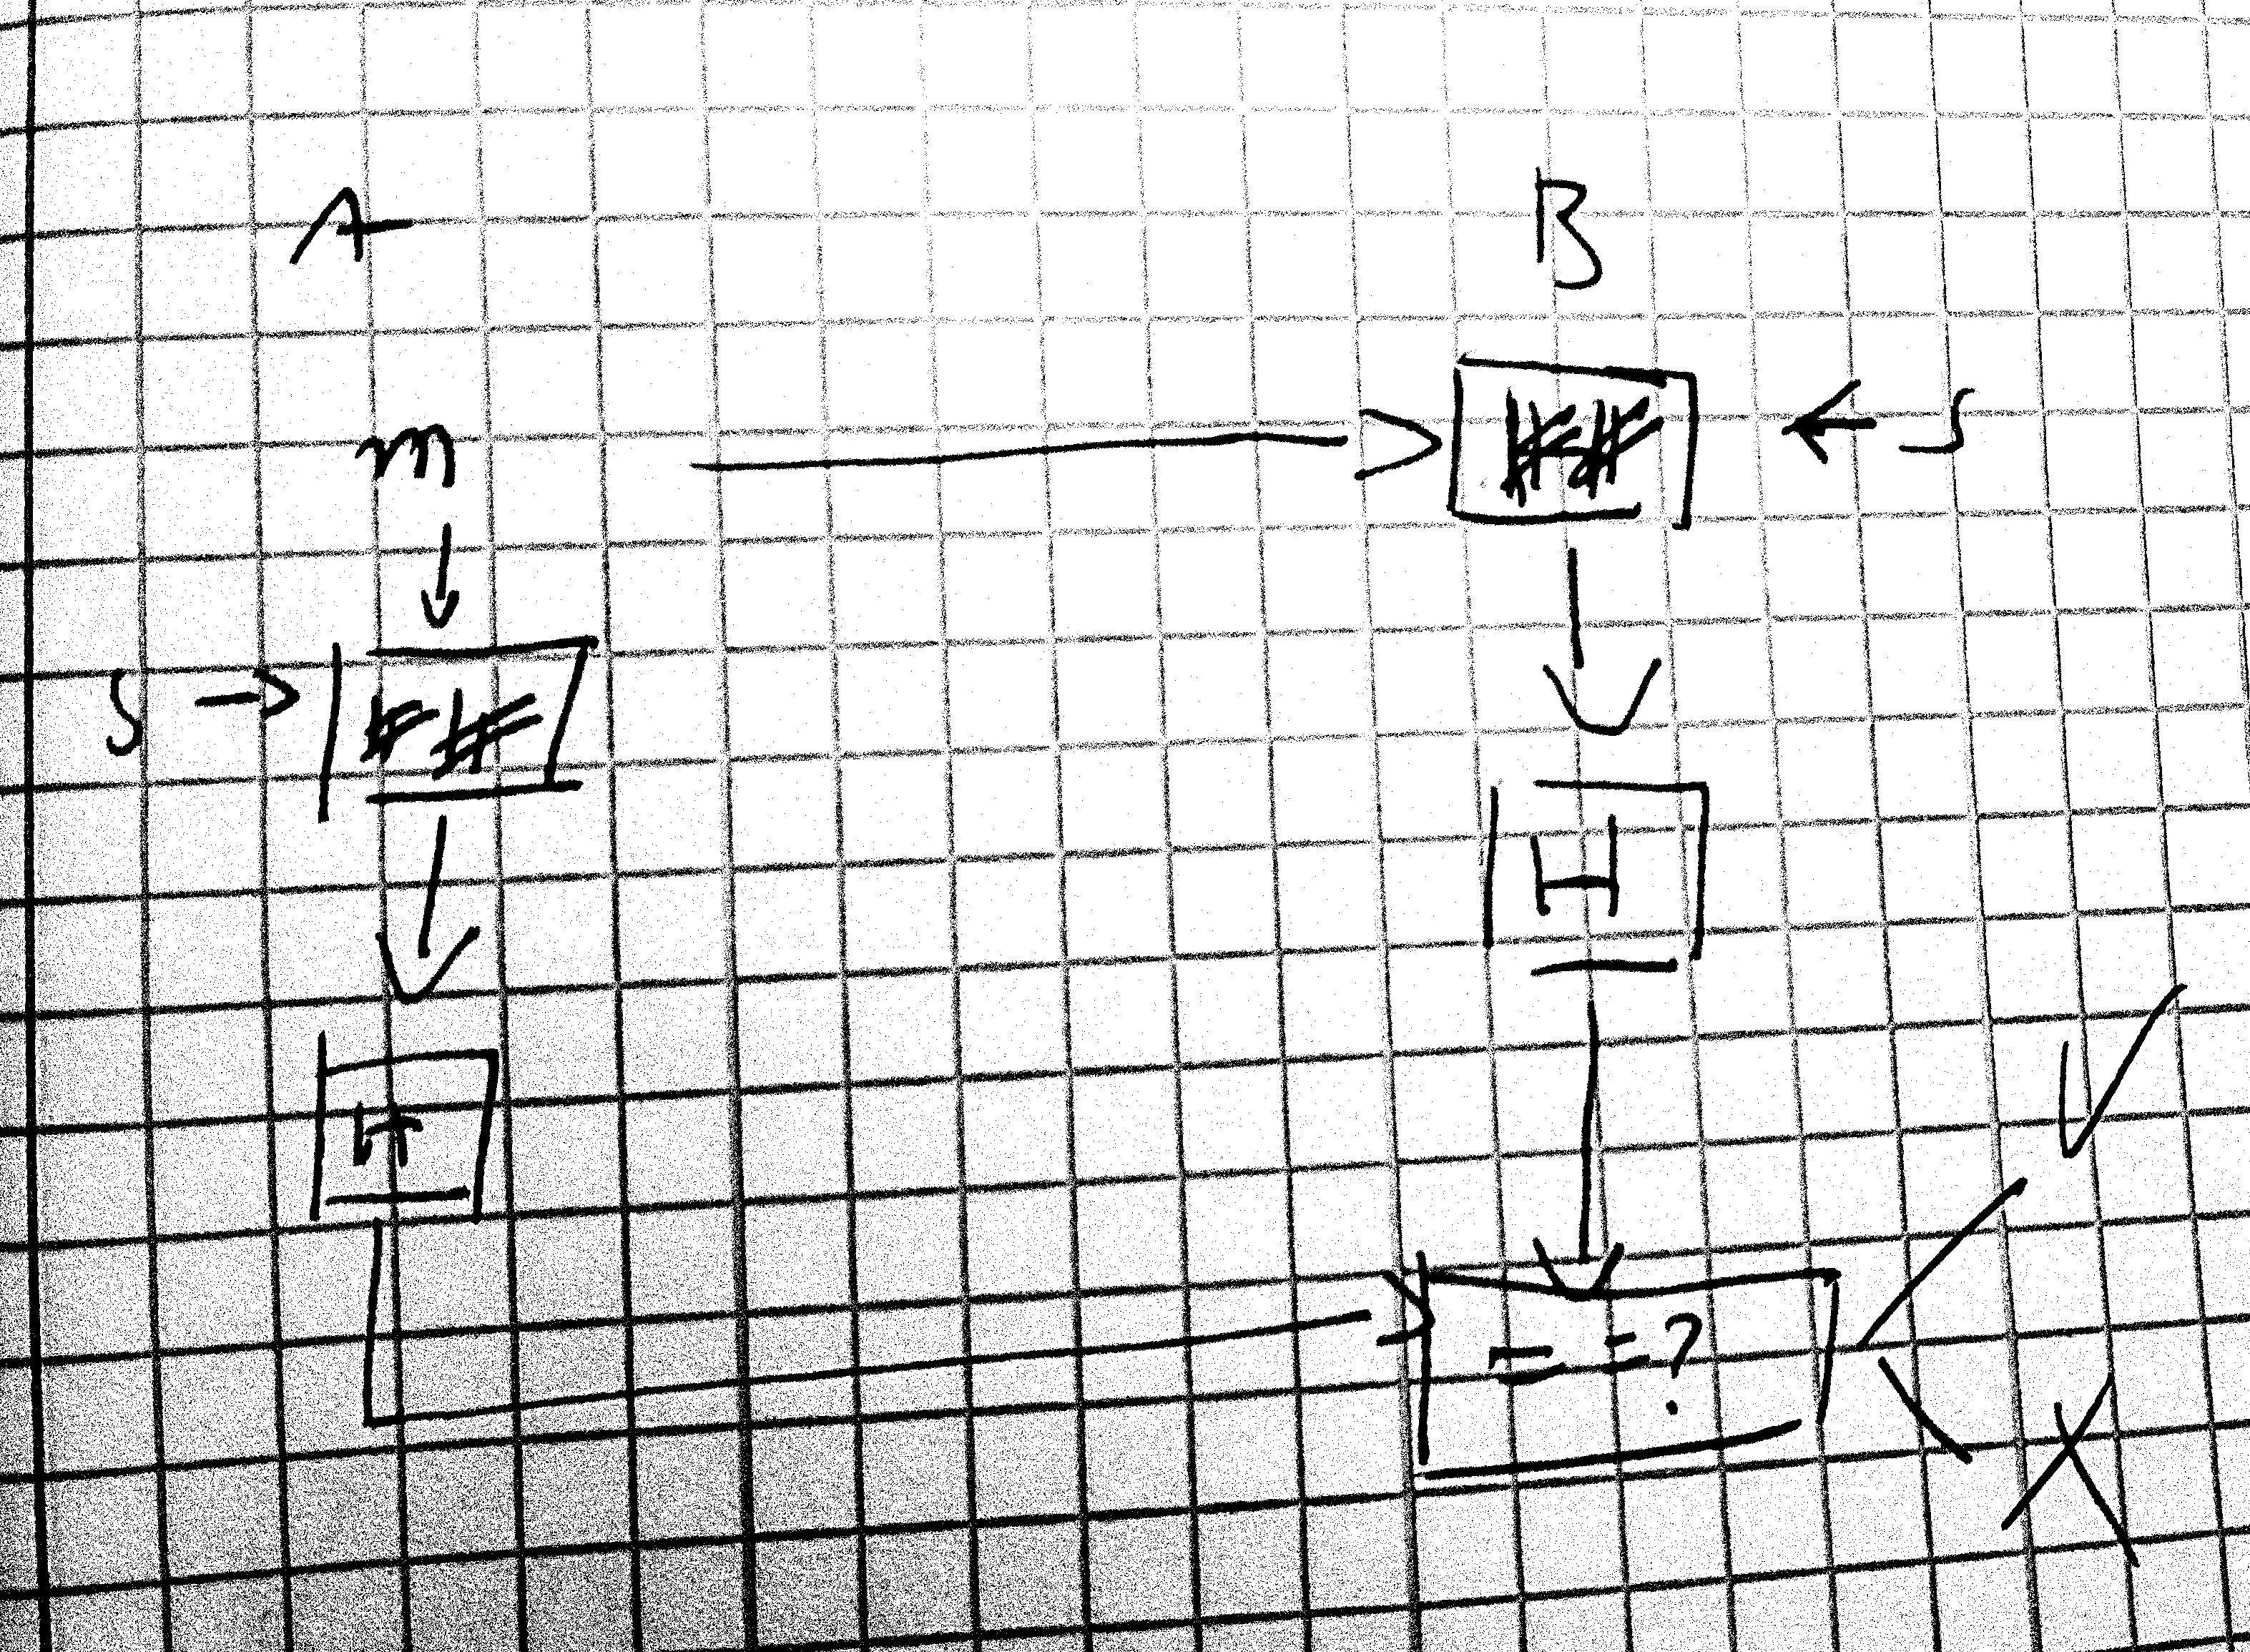
\includegraphics[width=0.6\textwidth]{authhash}

Per autenticare un documento in chiaro, le due soluzioni più diffuse sono HMAC e MAC.
	\begin{itemize}
		\item HMAC prevede che, per trasmettere un messaggio $m$ su un canale non affidabile, le due parti si accordino su un dato segreto $s$, una funzione hash sicura e una funzione di cifratura di $H(m)$ indicata con $HMAC(m, s)$.
Sul canale viene trasmesso $m \concat HMAC(m, s)$.
La destinazione suddivide il messaggio nelle due parti, calcola $HMAC(m, s)$ e ne verifica la congruenza.
\item MAC, invece, prevede che il messaggio $m$ venga cifrato secondo uno schema CBC con $IV = 0$ e che venga trasmesso sul canale non affidabile $m \concat MAC$, dove $MAC$ è l'ultimo blocco cifrato.
La destinazione effettua nuovamente la cifratura e quando lo desidera può controllare la congruenza di $MAC$.
HMAC è più efficiente data la maggiore efficienza delle funzioni hash.
La robustezza di HMAC e MAC è paragonabile.
MAC è poco utilizzato nella pratica perché il messaggio tende a diventare eccessivamente lungo.
	\end{itemize}
Sia HMAC che MAC lasciano aperto il problema del non ripudio, per risolvere il quale si usa la firma digitale.
Di seguito viene riportato lo schema di funzionamento di HMAC.
Lo schema di MAC ricalca quello di CBC.

\includegraphics[width=0.6\textwidth]{hmac}

\end{solution}
\part Si descriva il funzionamento delle firme digitali come sostituzione dell'autografo cartaceo.
\begin{solution}
Una firma digitale è un meccanismo crittografico atto ad assicurare autenticità e non ripudiabilità di un messaggio, ovvero a permettere al destinatario di essere certo che la sorgente non menta sulla propria identità e non possa negare la paternità del messaggio stesso.
Una firma digitale deve consentire a chiunque di identificare univocamente la sorgente del messaggio, non deve essere imitabile da impostori, non deve essere trasportabile da un documento all'altro, non deve essere ripudiabile e deve rendere evidenti eventuali alterazioni del documento a cui è apposta.
La sorgente deve quindi aggiungere informazioni non imitabili al messaggio che la destinazione sia in grado di verificare.
È possibile implementare una firma digitale con hash di un messaggio e un segreto, trasformazione $V/S$ o con cifrari simmetrici.

	Sei si utilizza un cifrario simmetrico, l'unico modo che si ha per costruire un sistema sicuro è quello di inserire una terza parte che funga da "notaio" e intervenga nel processo di firma tra le due entità in gioco.
	Questa terza parte viene chiamata \textit{registro degli atti privati} e genera una \textit{ricevuta}, che non può essere creata dalla sorgente né dalla destinazione e attesta l'integrità del messaggio.
	Se la funzione di cifratura è $E(\cdot)$, le entità in comunicazione sono $A, B$, la terza parte è $T$ e le due parti condividono con essa due chiavi $K_A, K_B$, il protocollo di firma è il seguente:
	\begin{enumerate}
		\item $A \rightarrow T: E_{K_A}(m \concat A)$
		\item $T$ genera una chiave $R$ e la usa per criptare una ricevuta $r = E_R(m \concat A \concat T)$
		\item $T \rightarrow A: E_{K_A}(A \concat T \concat m \concat r)$
		\item $A$ controlla che $m$ non sia stato modificato
		\item $A \rightarrow B: m \concat A \concat T \concat r$
		\item $B \rightarrow T: m \concat A \concat T \concat r \concat B$
		\item $T$ controlla la validità di $r$
		\item $T \rightarrow B: E_{K_B}(T \concat A \concat m)$
	\end{enumerate}
Questo modello comporta un enorme sforzo computazionale per $T$ e quindi non viene usato per la pratica, dato che richiede che $T$ sia sempre online e si comporti correttamente.

Nel caso di una trasformazione $S(\cdot)$ applicata allo hash del messaggio $m$ la destinazione deve ricevere di una funzione di verifica $V(\cdot)$ tale che, se la firma è valida, valga $V(S(H(m))) = H(m)$.
È importante, in questo caso, che $H(\cdot)$ abbia la proprietà di resistenza alle collisioni, per evitare che due messaggi abbiano hash uguali.
Se si usa lo hash $H(m\concat s)$ costituito dallo hashing della concatenazione tra il messaggio $m$ e un segreto $s$, invece, entrambe le parti devono conoscere il segreto $s$ in modo che la destinazione possa calcolare in autonomia $H(m\concat s)$.
Questo metodo, quindi, non garantisce la non ripudiabilità ed è utile se le due parti si fidano l'una dell'altra.
È importante la proprietà di unidirezionalità di $H(\cdot)$ per evitare che una terza parte possa risalire a $s$ a partire da un messaggio intercettato e poter quindi produrre hash per messaggi arbitrari.
\end{solution}
\part Si descriva il protocollo sfida/risposta unilaterale. Nel caso dell'uso di cifrari simmetrici è possibile usare sia cifrari a flusso che cifrari a blocchi? Nel caso dell'uso di cifrari a blocchi, quali modalità di cifratura è opportuno adottare?
\begin{solution}
	Il protocollo sfida/risposta è una contromisura all'attacco con replica che prevede che la prova d'identità sia continuamente cambiata, soddisfando la regola secondo cui il calcolo dell aprova di identità da fornire deve essere facile per chi conosce una informazione segreta e difficile per chi dispone solo delle prove inviate in precedenza.
	È possibile costruire un protocollo di sfida e risposta in tre modi: mediante l'uso di funzioni hash, di un cifrario, o di firma dgitale.
	Se si usano funzioni hash, le due parti concordano una funzione $H(\cdot)$ crittograficamente sicura e un segreto $s$.
	Quando si richiede l'identificazione di $A$ da parte di $B$ si esegue il seguente protocollo a tre passi:
	\begin{enumerate}
		\item $B \rightarrow A: R_B$, con $R_B$ dato di sfida mai usato prima (detto nonce)
		\item $A \rightarrow B: c = H(R_B \concat s)$
		\item $B$ calcola $c$ e verifica la congruenza.
	\end{enumerate}
	Di seguito è riportato lo schema di questo protocollo.

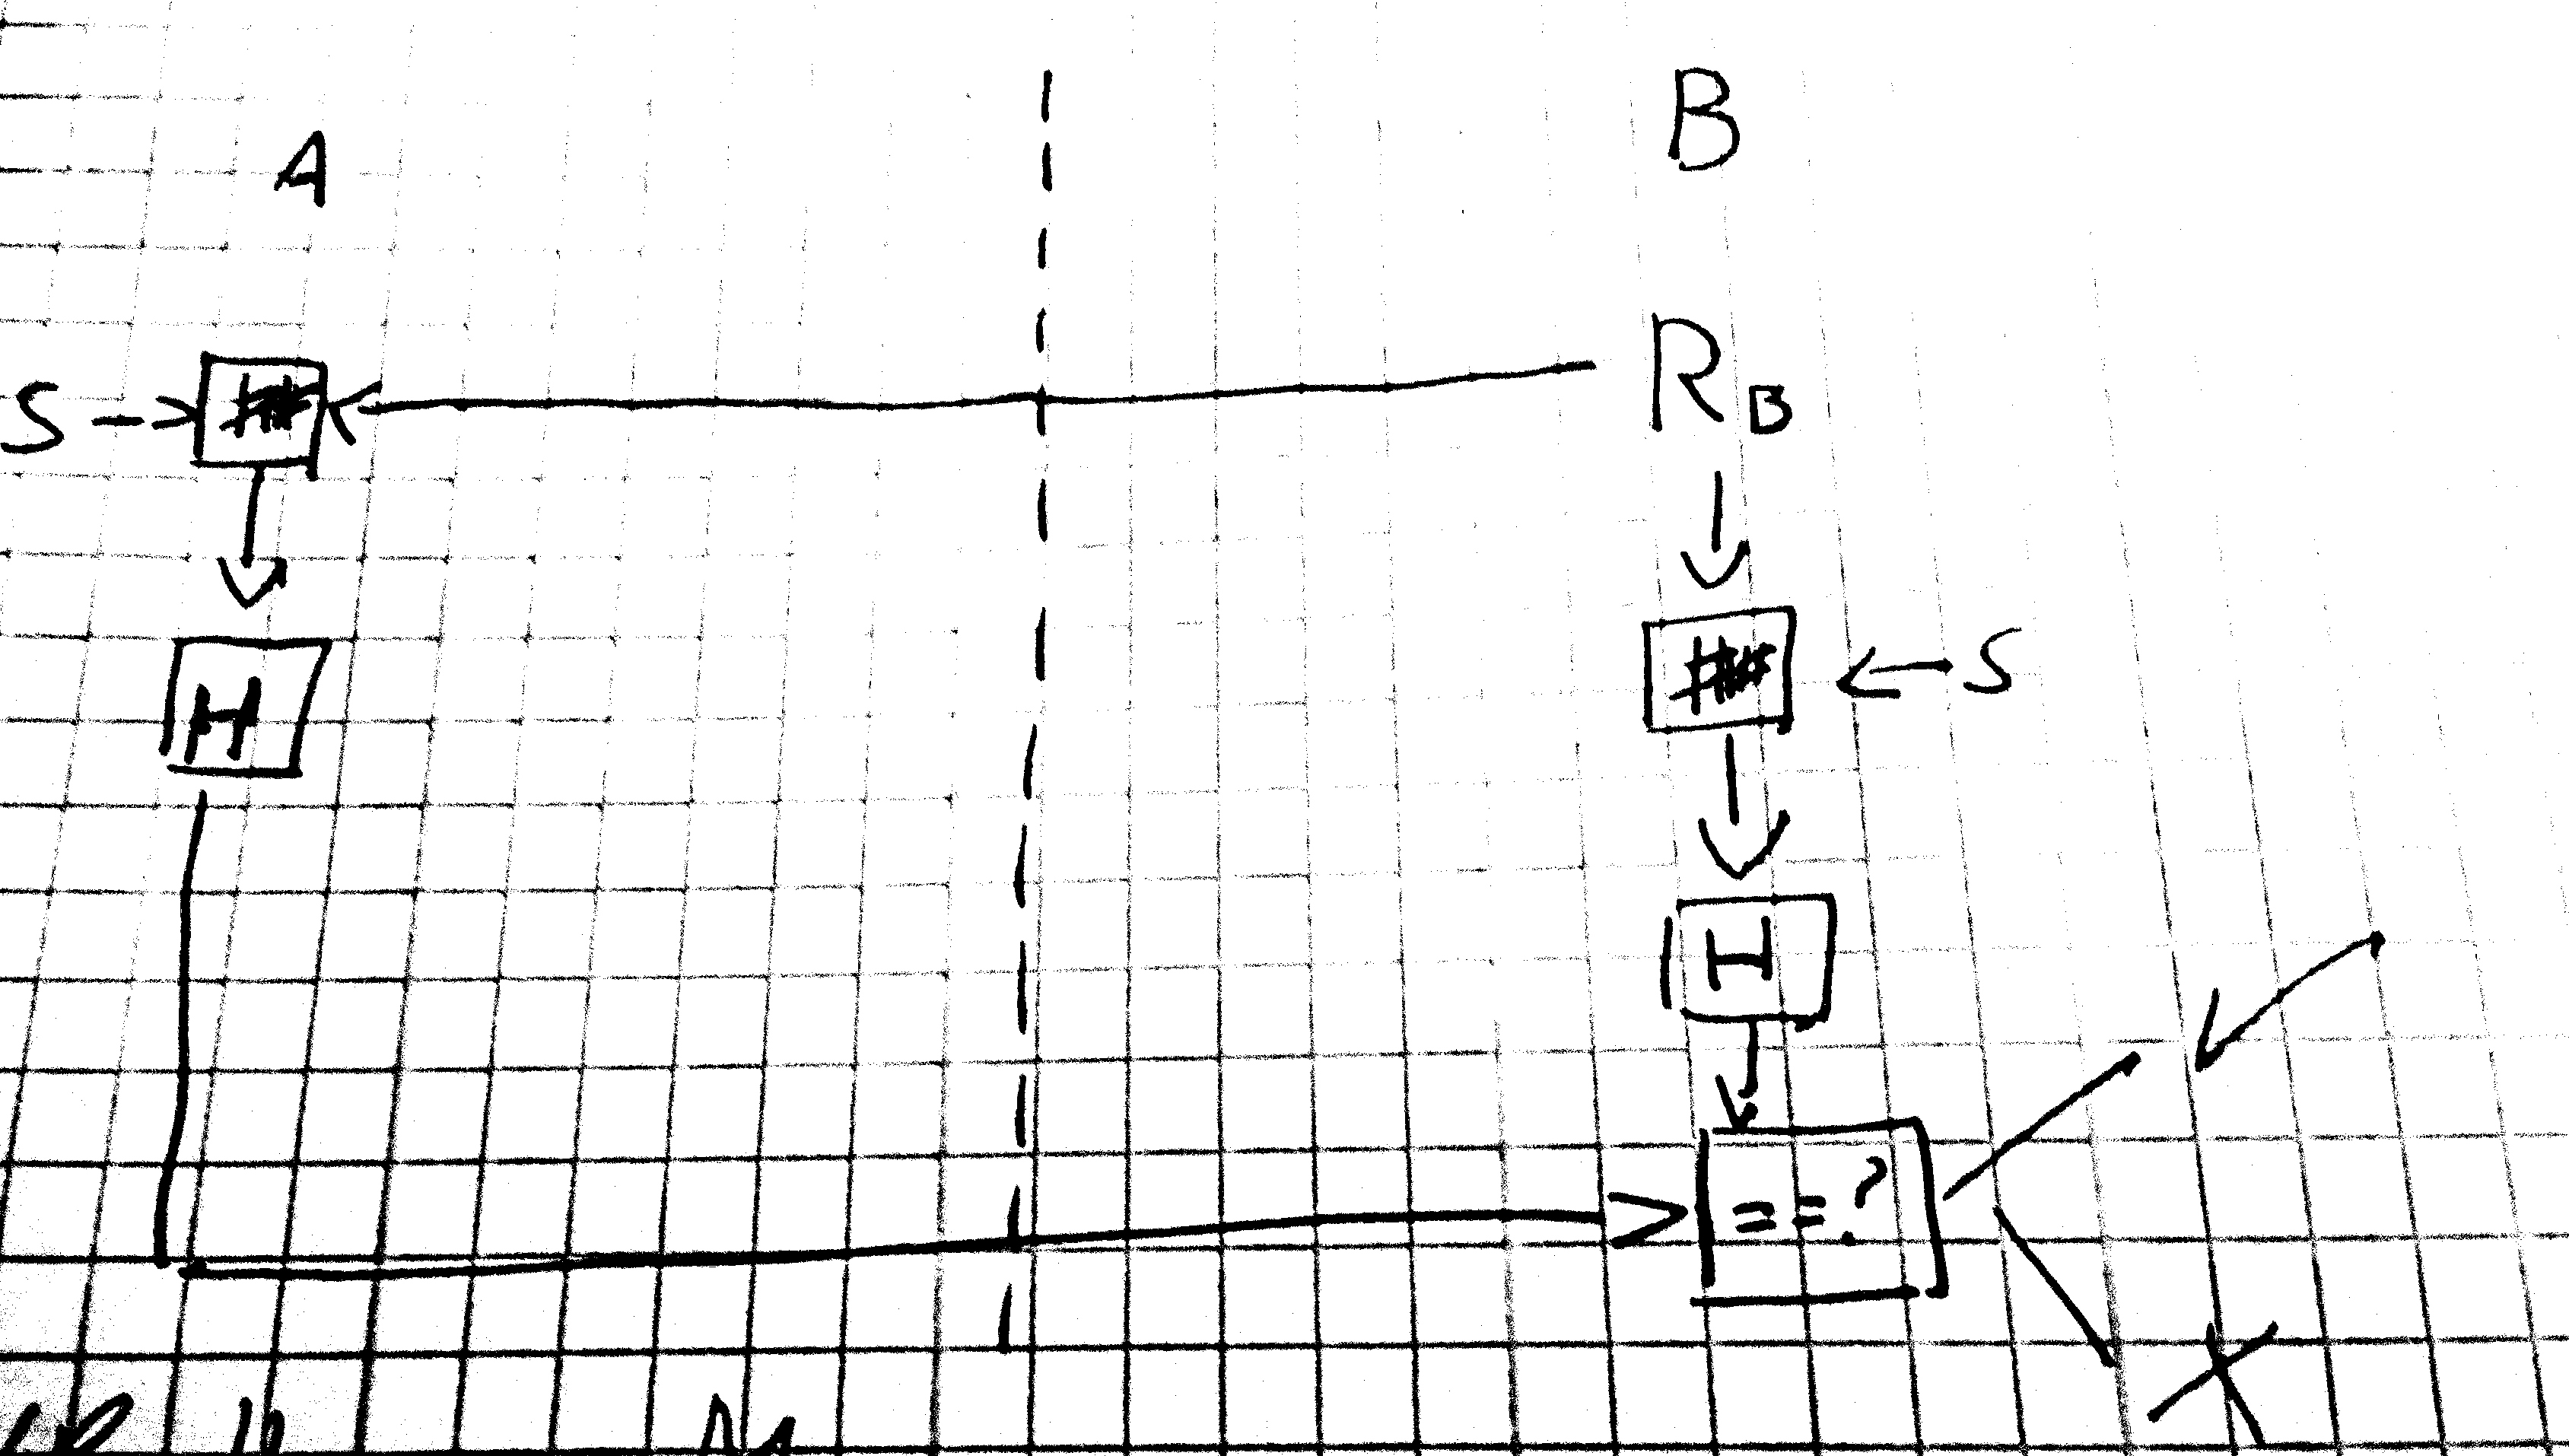
\includegraphics[width=0.6\textwidth]{crhash}

	Se si vuole mutua identificazione occorrono due dati di sfida $R_A, R_B$ e il protocollo viene così modificato:
	  \begin{enumerate}
    \item $B \rightarrow A: R_B$, con $R_B$ dato di sfida mai usato prima (detto nonce)
    \item $A \rightarrow B: c_A = R_A \concat H(R_B \concat s)$
		\item $B \rightarrow A: c_B = H(R_A \concat s)$
		\item $A, B$ calcolano $c_B, c_A$ e verificano la congruenza
  \end{enumerate}
	Di seguito è riportato lo schema di questo protocollo.

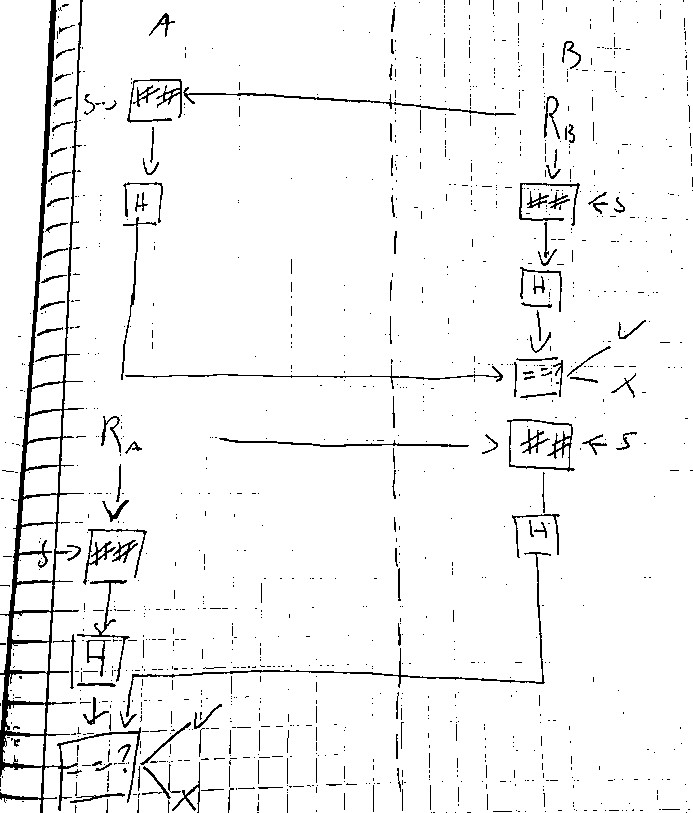
\includegraphics[width=0.6\textwidth]{crhashmut}

	Questo protocollo è però vulnerabile all'attacco del gran maestro di scacchi (interleaving), nel quale un intrusore intercetta le comunicazioni in una direzione e nell'altra e le usa per identificarsi con entrambe le parti, e agli attacchi di reflection, nel quale un intruso apre una sessione di sfida e una di risposta con lo stesso utente.
	Per evitare attacchi di replay e interleaving ci si serve di timestamp, che devono essere forniti però da un servizio sicuro; per evitare attacchi di interleaving si possono usare dei numeri di sequenza, che però devono essere memorizzati e sono problematici in reti poco affidabili; per evitare attacchi di reflection si inserisce nei messaggi l'identificatore del mittente, ottenendo il seguente protocollo:
	  \begin{enumerate}
    \item $B \rightarrow A: R_B$, con $R_B$ dato di sfida mai usato prima (detto nonce)
    \item $A \rightarrow B: c_A = R_A \concat H(R_A \concat R_B \concat \concat B \concat s)$
		\item $B \rightarrow A: c_B = H(R_A \concat R_B \concat A \concat s)$
		\item $A, B$ calcolano $c_B, c_A$ e verificano la congruenza
  \end{enumerate}
	È possibile implementare il protocollo sfida/risposta anche con cifrari simmetrici.
	In questo caso il verificatore cifra il nonce, riceve la sua decifratura e confronta il risultato con il dato che ha generato.
	La segretezza della funzione $D$ impedisce a un intruso di rispondere alla sfida, la variazione di $r$ rende inutile intercettazione e replica; in ogni caso, il timestamp è comunque utile.
	Di seguito è riportato lo schema di questo protocollo.

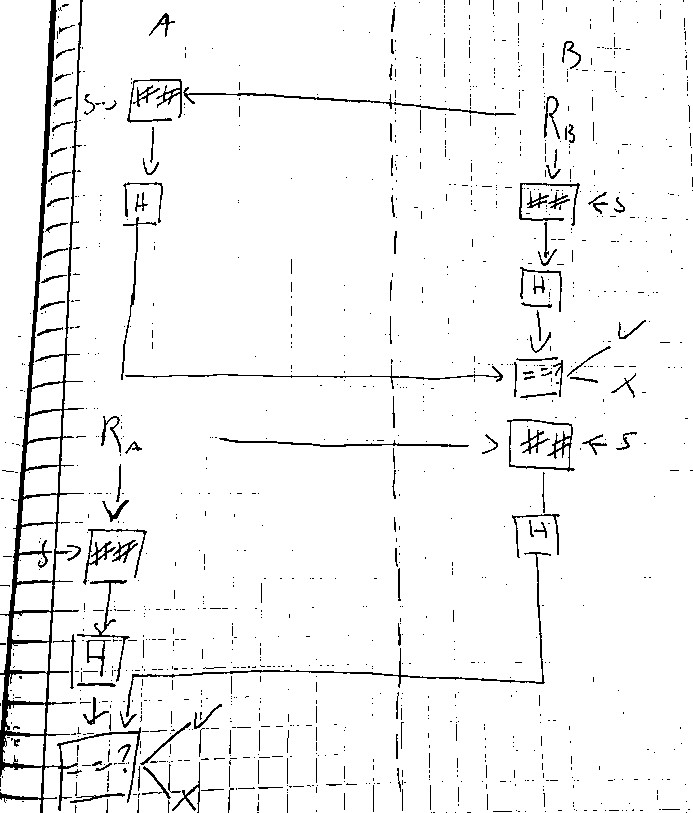
\includegraphics[width=0.6\textwidth]{crhashmut}

	È inoltre possibile implementare una sfida/risposta con uno schema di firma digitale, nel qual caso il verificatore trasmette il nonce in chiaro, lo riceve firmato e verifica la firma.
	Di seguito è riportato lo schema di questo protocollo.

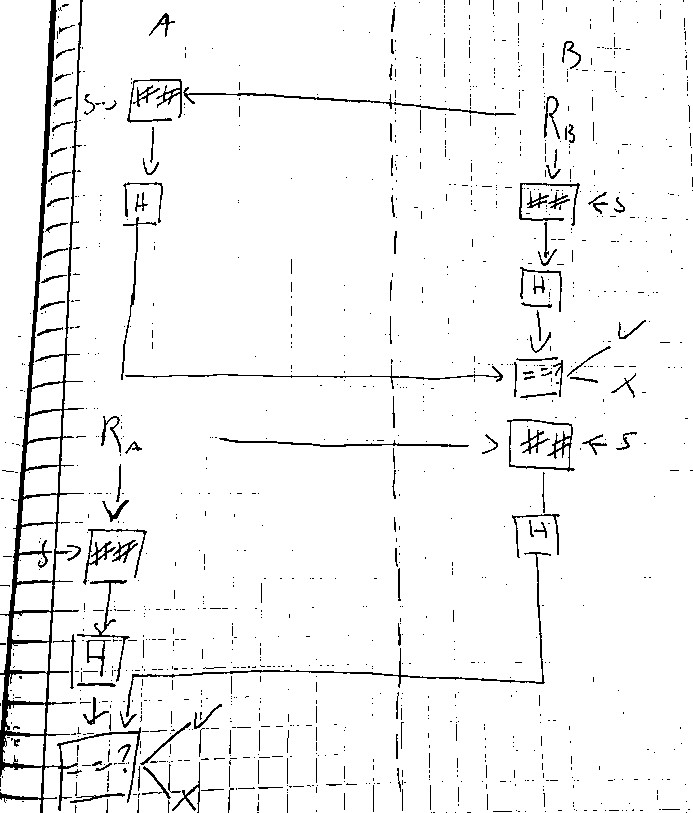
\includegraphics[width=0.6\textwidth]{crhashmut}

\end{solution}
\part Si descrivano i modelli di distribuzione di chiavi (KA, Key Agreement) Master Key, KDC e DH servendosi di opportuni schemi.
\begin{solution}
Il modello di distribuzione master key prevede che ci sia un mutuo accordo tra tutte le possibili coppie di utenti A e B su una chiave $AB$, detta master key, che viene utilizzata solo per cifrare le chiavi di sessione $k$ generate tramite PRNG all'avvio di una sessione.
Ogni chiave di sessione viene usata per cifrare una sola comunicazione tra A e B, e comunicata cifrandola con la master key.
È possibile cifrare le chiavi di sessione con ECB perché il dato è aleatorio: usando CBC, la necessità di padding rallenterebbe il processo.
Il modo più sicuro di usare la chiave di sessione è usarla una volta sola.
Ogni tanto, la master key deve comunque essere rinnovata mediante un incontro personale o un corriere fidato.
Il modello master key richiede la generazione di $\Sigma (n - 1)$ chiavi, il che rende apparenti i problemi di scalabilità di questo sistema.
Di seguito viene riportato lo schema di funzionamento di questo modello.

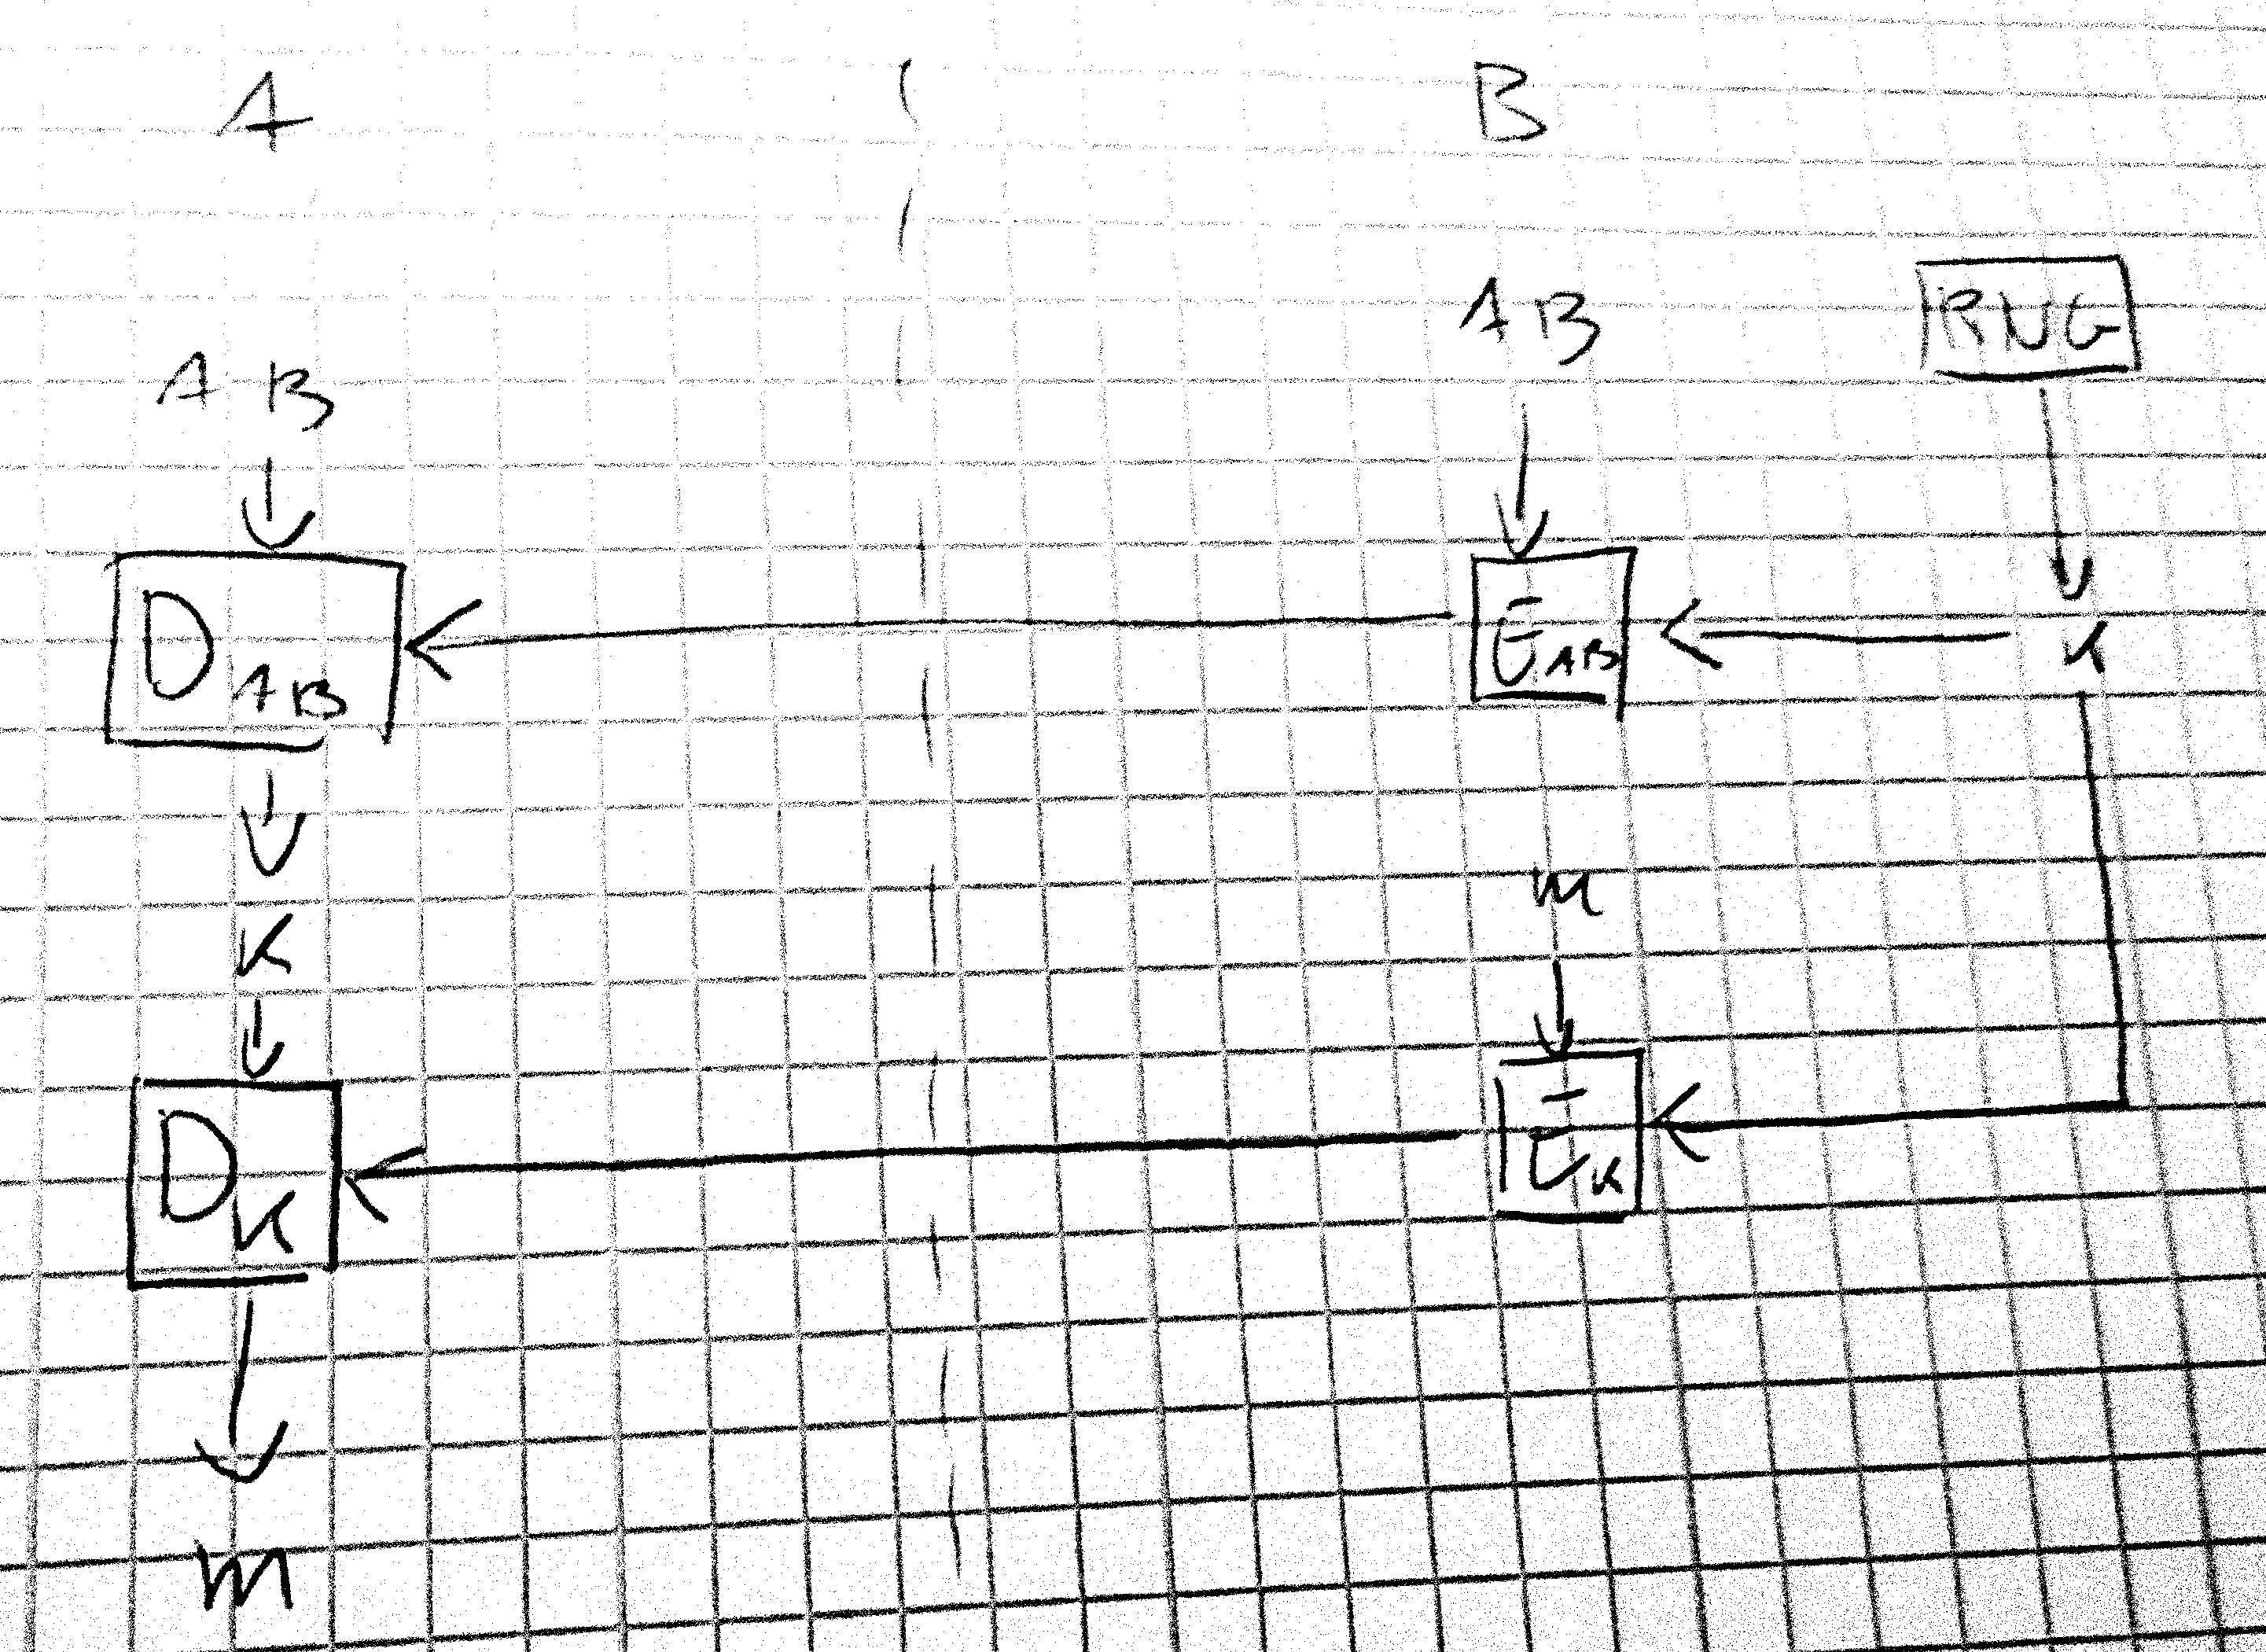
\includegraphics[width=0.6\textwidth]{masterkey}

Il modello a centro di distribuzione di chiavi (KDC) prevede che un'autorità centrale, il KDC appunto, sia responsabile per la generazione e l'invio delle chiavi di sessione.
In questo modo l'autorità centrale deve memorizzare solamente un numero di chiavi pari al numero di utenti.
Questo modello prevede il seguente protocollo per l'avvio di una comunicazione tra due parti $A, B$ che hanno concordato due chiavi $K_A, K_B$ con una terza parte fidata $T$:

	\begin{enumerate}
		\item $A \rightarrow T: R_A \concat A \concat B$
		\item $T \rightarrow A: E_{K_A}(R_A\concat B \concat k \concat E_{K_B}(A \concat k))$
		\item $A \rightarrow B: E_{K_B}(A\concat k)$
		\item $B \rightarrow A: E_k(R_B)$
		\item $A \rightarrow B: E_k(R_B - 1)$
	\end{enumerate}

Gli ultimi due passi servono a evitare un attacco con replica. 
Se mancassero un intruso potrebbe ripresentare il terzo messaggio un numero arbitrario di volte, forzando $B$ a mandare messaggi arbitrari cifrati con $k$, riducendo quindi il livello di sicurezza.
Se invece un intrusore riuscisse a decifrare $k$ (cosa improbabile) potrebbe impersonare $A$ e catturare ogni informazione inviata successivamente, se $k$ viene riutilizzata.
	Per contrastare questo attacco, $B$ può mantenere uno storico delle chiavi utilizzate ed evitare di riutilizzarle, oppure il KDC può attribuire un tempo di vita limitato a ogni chiave di sessione (questo è il comportamento di Kerberos).
	KDC è molto gravoso per  terza parte, alla quale è richiesto di essere sempre online, di non rappresentare un collo di bottiglia, di essere degna di fiducia e, se si prevede un sistema di \textit{key recovery}, si memorizzare le chiavi su una memoria sicura. 

Di seguito viene riportato lo schema di funzionamento di questo modello.

\includegraphics[width=0.6\textwidth]{kdc}

Il modello Diffie-Hellman (DH) anonimo non richiede una terza parte né una master key: è un algoritmo anonimo che permette a due parti di accordarsi per una chiave di sessione.
Le due parti generano due numeri $x_A, x_B \in 1..p-1$, essendo $p$ un numero primo.
Ognuna delle due calcola poi $y = F(x)$, con $F(\cdot)$ unidirezionale, e invia $y$ sul canale insicuro.
Una volta avvenuto lo scambio, le due parti devono disporre i una funzione $G(\cdot)$ tale che $G(x_A, y_B) = G(x_B, y_A) = k$.
Diffie e Hellmann, nel loro articolo, suggeriscono l'esponenziazione modulare, ovvero
\begin{equation}
\begin{array}{ll}
y = F(x) &= g^x \mod p \\
k = G(x, y) = y^x \mod p
\end{array}
\end{equation}
dove $g < p$ è un generatore del campo di Galois $GF(p)$, ovvero un numero le cui potenze modulo $p$ forniscono una permutazione di $Z^*_p$.
$k$ è detto \textit{pre-master secret}.
$p$ e $g$ non sono segreti e devono essere noti: possono essere stabiliti da un'autorità o semplicemente comunicati all'inizio del primo messaggio.
Ottenere $k$ partendo solo da un $x$ corrisponde al problema del logaritmo modulare, computazionalmente molto difficile.
Il modello DH non fornisce alcuna garanzia di autenticità, dato che i numeri non contengono informazione sulla propria origine: ognuna delle due parti potrebbe essere un intruso.
Per questo motivo, lo scambio appena descritto è noto anche come DH anonimo.
Di seguito viene riportato lo schema di funzionamento di questo modello.

\includegraphics[width=0.6\textwidth]{dh}

Una variante di DH prevede che l'iniziatore del protocollo abbia a disposizione $y_B$ ottenuto in precedenza e in modo sicuro, perdendo chiaramente tuttavia la possibilità di comunicare senza accordi fuori banda.
In questo caso è sufficiente inviare $y = g^r \mod p$, con $r$ casuale, per generare il segreto one-time $k = g^{rx} \mod p$.
\end{solution}
\part Si descrivano i modelli di scambio di chiavi Diffie-Hellman anonymous, fixed ed ephemeral. Si disegni uno schema del funzionamento. In che modo si può rendere più efficiente il calcolo del coefficiente pubblico $Y$ nello scambio DH?
\begin{solution}
Lo scambio di chiavi DH anonimo (descritto nella domanda relativa allo scambio DH, ndr) non prevede autenticazione delle due parti.
Se si richiede autenticazione è possibile servirsi dello scambio fixed o dello scambio ephemeral.
Lo scambio fixed prevede che si ottenga da una CA un certificato sui parametri pubblici $y_A, y_B$, che vengono fissati e rimangono sempre uguali.
In questo modo però, per evitare che il pre-master secret sia sempre uguale, vengono generati e scambiati due nonce (numeri casuali usati una sola volta) $R_A, R_B$ e il segreto comune (master secret) viene calcolato come $H(R_A \concat R_B \concat k)$.
Di seguito è riportato lo schema di funzionamento dello scambio DH fixed.

\includegraphics[width=0.6\textwidth]{dhfixed}

Lo scambio ephemeral, invece, prevede che le due parti dispongano di una chiave pubblica certificata e i parametri pubblici $y_A, y_B$ siano firmati digitalmente in modo da garantire autenticità.
In ogni caso, per mantenere la compatibilità con il DH fixed, vengono comunque usati due nonce per generare il master secret.
Di seguito è riportato lo schema di funzionamento dello scambio DH ephemeral.

\includegraphics[width=0.6\textwidth]{dhephemeral}

È possibile rendere più efficiente il calcolo di $Y$ mediante la tecnica del "repeated square and multiply", un metodo generale per calcolare rapidamente potenze intere arbitrarie di un numero.
\end{solution}
\end{parts}
\question \textbf{Cifrari asimmetrici, cifrari ibridi e meccanismi asimmetrici di autenticazione. Firma digitale con meccanismi asimmetrici}
\begin{parts}
\part Perché può essere utile usare due chiavi differenti, una pubblica e una privata? Quali sono i possibili attacchi a cui è suscettibile un modello di questo tipo?
\begin{solution}
In un sistema asimmetrico, nel quale per firmare o criptare un messaggio si utilizza una chiave diversa da quella usata per verificare una firma o decriptare un messaggio, è risolto il problema dello scambio di chiavi che tradizionalmente deve avvenire attraverso un canale sicuro.
La chiave pubblica, infatti, può essere diffusa senza timori, e solo quella privata deve essere tenuta segreta.

	I sistemi asimmetrici sono vulnerabili ad attacchi di vari tipi: brute-force, che tuttavia è impraticabile data una chiave sufficientemente lunga; matematici, come ad esempio, nel caso di RSA, la fattorizzazione di $n$ nei suoi fattori primi, la quale però nuovamente è impraticabile se $n$ è sufficientemente grande; a tempo, i quali si basano sul legame tra la chiave privata e il tempo impiegato per decifrare un messaggio, e possono essere combattuti con una tecnica chiamata \textit{blinding}; a testo cifrato scelto, che sfruttano la caratteristica di determinismo e si combattono rendendo il cifrario probabilistico; man-in-the-middle, che possono essere combattuti tramite una terza parte fidata che certifica l'autenticità della chiave pubblica.
\end{solution}
\part Si enuncino le formule per generare il testo cifrato a partire dal testo in chiaro e viceversa usando RSA.  Si discutano la robustezza di RSA, i possibili attacchi e le possibili soluzioni.
\begin{solution}
La trasformazione operata sul testo in chiaro $m$ è $c = m^e \mod n$, in cui $n = p q$, $p$ e $q$ sono primi ed $e$ è coprimo con $\Phi(n) = (p - 1) (q - 1)$.
La trasformazione operata sul testo cifrato è $c^d \mod n = (m^e \mod n)^d \mod n = m^{ed} \mod n = m$.
Ciò vale perché $e$ e $d$ sono scelti in modo tale che
\begin{equation}
m^{ed} \mod n = m \forall m \in 0..(n - 1)
\label{eq:rsa}
\end{equation}
Scegliere tre interi $n, e, d$ tale che valga la \cref{eq:rsa} è computazionalmente facile.
La chiave pubblica è costituita dalla coppia $(e, n)$, mentre la chiave privata è costituita dalla coppia $(d, n)$.
	La sicurezza di RSA è garantita dalla difficoltà del calcolo della radice $e$-esima $\sqrt[e]{c}$ in mancanza della trapdoor $d$ che permette di sfruttare la trasformazione riportata sopra.
	Se si conosce solo la chiave pubblica è possibile in linea di principio dedurre la chiave privata fattorizzando $n$ e calcolando $\Phi(n)$ e $d = e^{-1} \mod \Phi(n)$; questo attacco è però computazionalmente impossibile se i primi sono molto grandi.
	Se un messaggio è relativamente corto diventano fattibili vari tipi di attacchi: in primis il brute force, che richiederebbe tantissimo tempo se il messaggio fosse più lungo, ma anche attacchi di tipo replay.
La soluzione è l'uso di padding: può essere allegato al messaggio un numero pseudo-casuale $r$, in modo da identificare univocamente il messaggio e allungarlo, o servirsi dell'Optimal Asymmetric Encryption Padding.
L'OAEP trasforma RSA in un cifrario probabilistico: servendosi di un intero casuale $r$ e due funzioni hash $H_1, H_2$, il messaggio $m$ viene trasformato in $00\concat X\concat(r \oplus H_2(X)), X = m\concat H_1(r)$, che contiene un elemento di casualità.
OAEP oltre a garantire casualità dell'uscita è una contromisura per gli attacchi a testo cifrato scelto.
Di seguito viene riportato uno schema del funzionamento dell'OAEP, che segue lo schema della rete di Feistel.

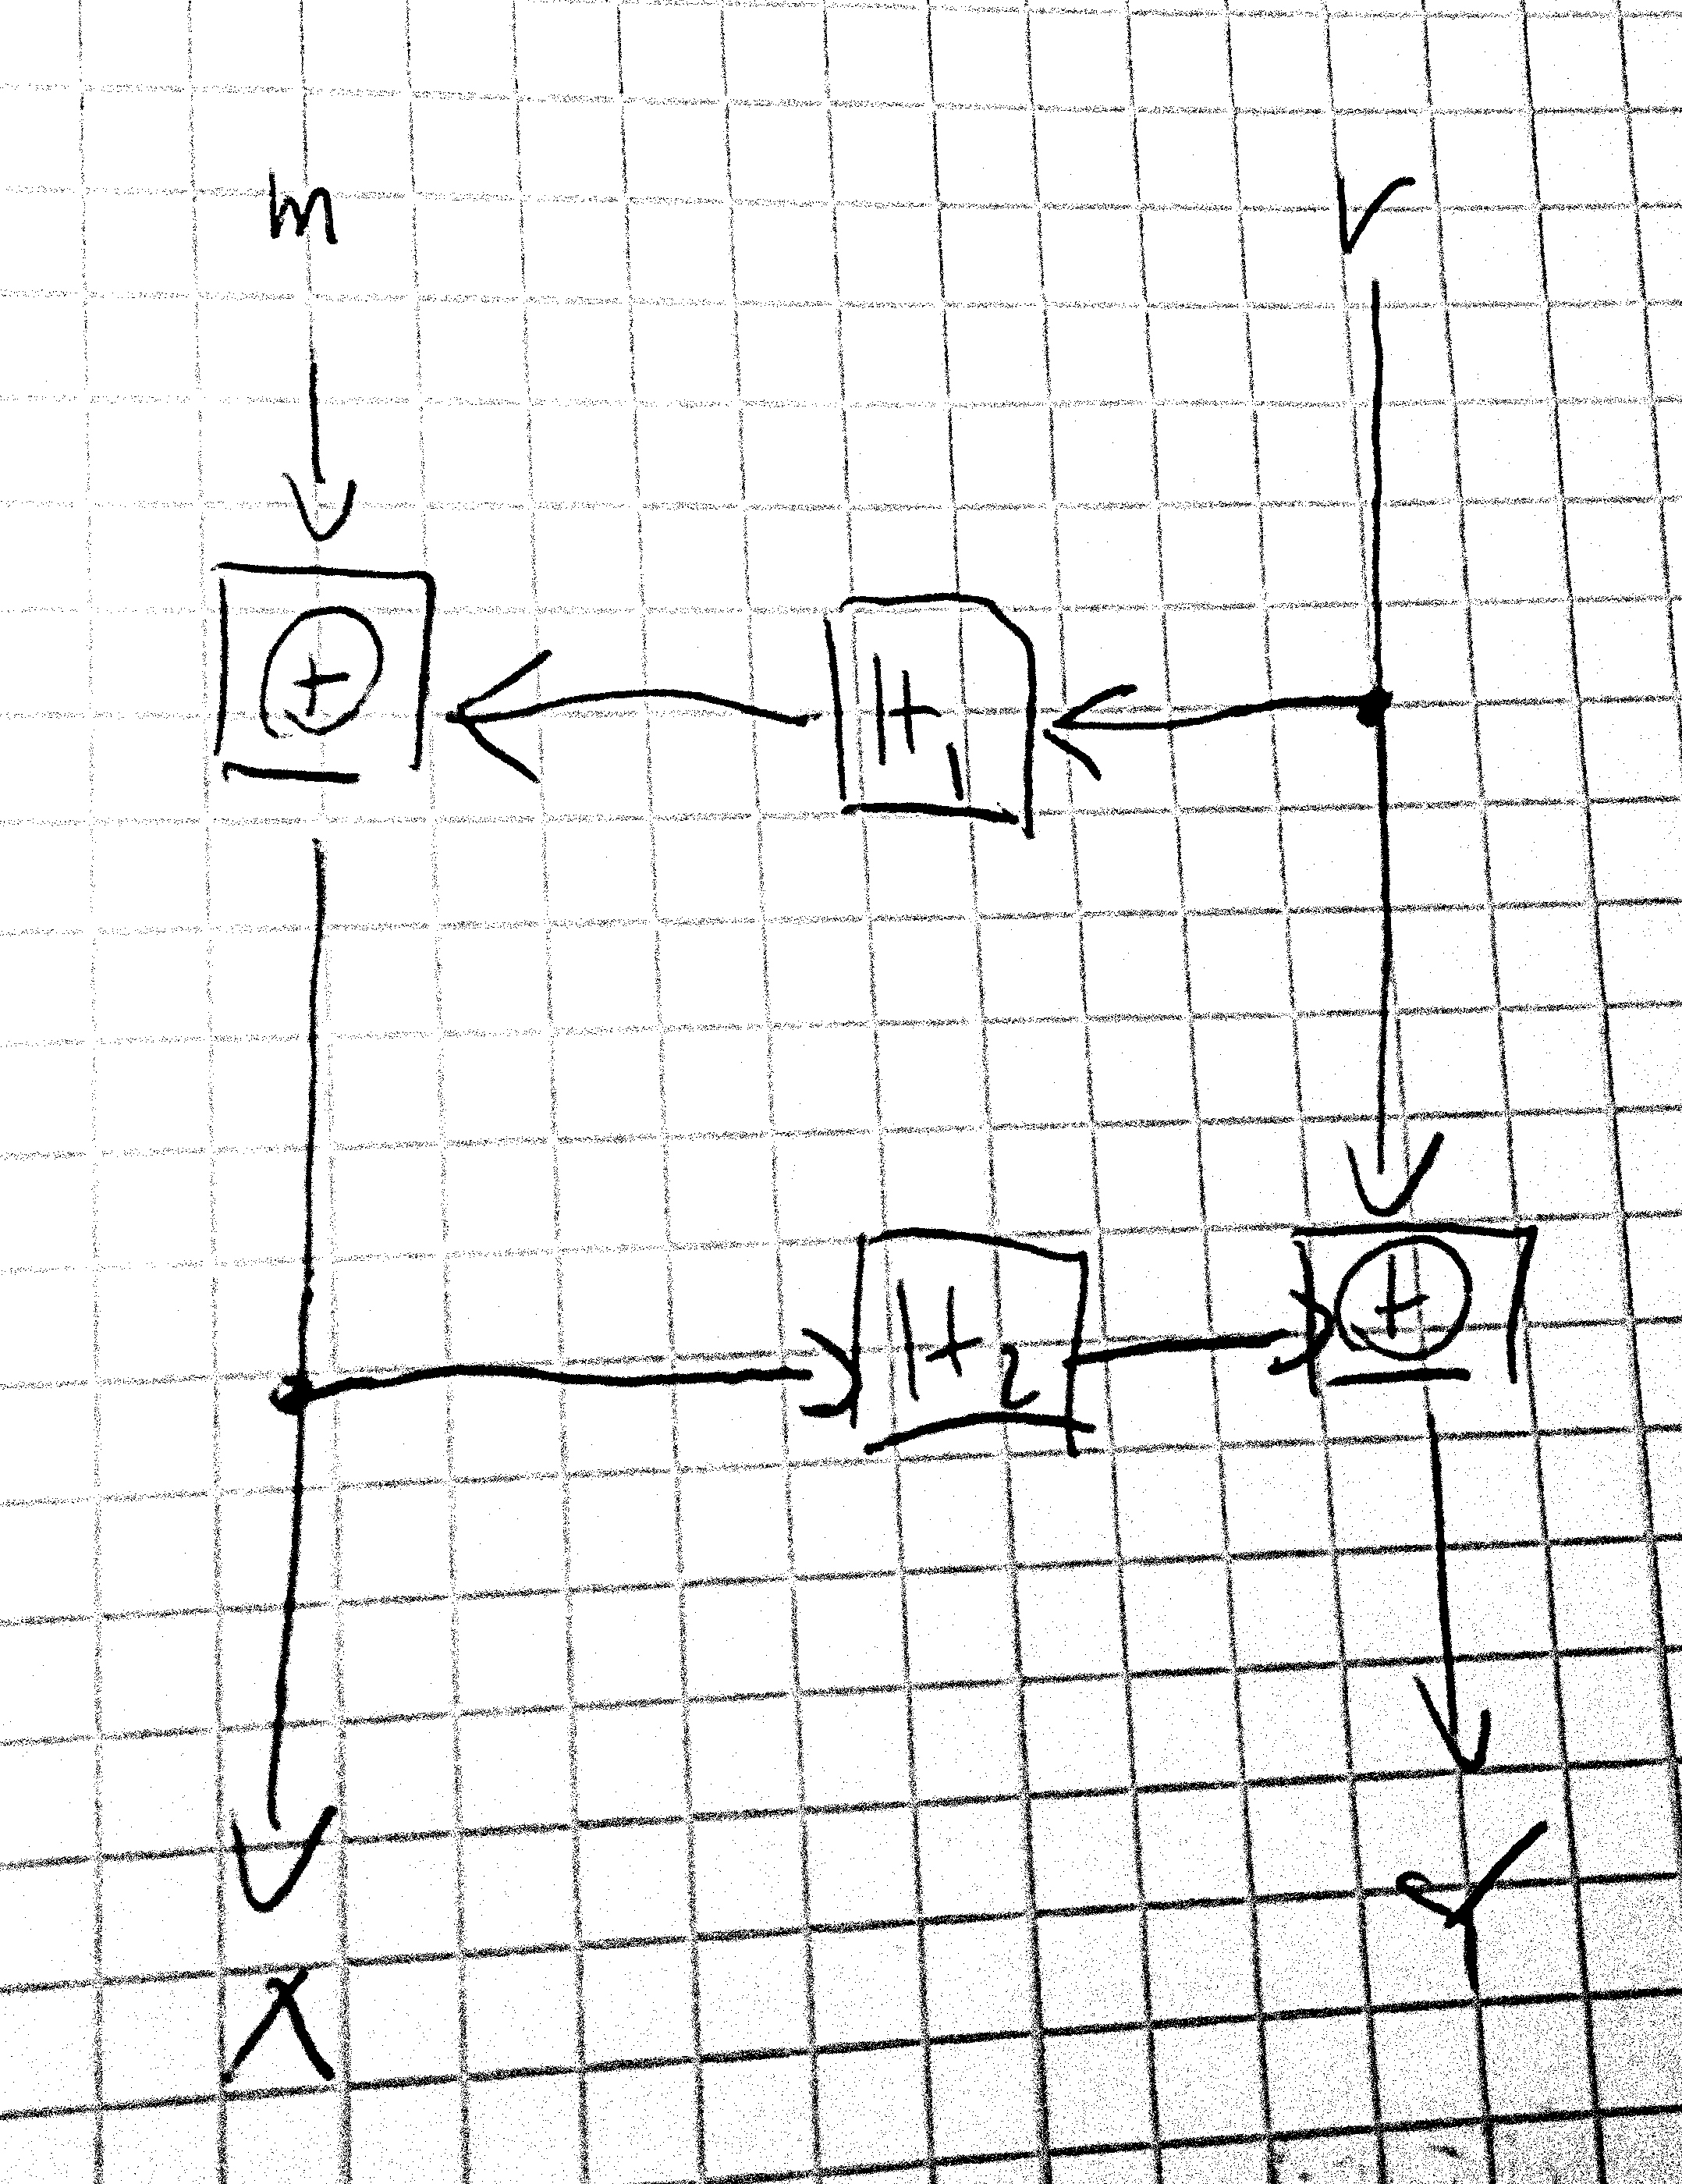
\includegraphics[width=0.6\textwidth]{oaep}

\end{solution}
\part Si descriva il processo di firma con RSA. Perché una firma con recupero non può avere valore legale? Si descrivano i pro e i contro della firma recupero e appendice.
\begin{solution}
Gli algoritmi asimmetrici di firma si distinguono in firma con recupero e firma con appendice.
Gli algoritmi di firma con appendice prevedano che venga criptato con la chiave privata della sorgente lo hash $H(m)$, con $H(\cdot)$ crittograficamente sicura, e che $E(H(m))$ venga allegato al messaggio.
La sorgente decripta la firma, calcola l'impronta del messaggio ricevuto e verifica la congruenza.
Gli algoritmi di firma con appendice richiedono il messaggio originale per verificarne l'autenticità.
La firma con appendice permette di rispettare il requisito di non trasportabilità e quello di non alterabilità.
Sottoponendo un messaggio di un documento a una funzione hash un intrusore non è in grado di trasportare la firma su un altro documento perché, chiaramente, lo hash sarà diverso; lo stesso vale in caso di alterazione del messaggio.
	Gli algoritmi di firma con recupero dividono il messaggio $m$ in più blocchi $m_i$ tali che $m_i < n$.
A quel punto ogni blocco è trasformato con una funzione $R(\cdot)$ invertibile e poi criptato usando la chiave privata della sorgente.
La destinazione decripta i blocchi usando la chiave pubblica della sorgente, verifica se il risultato appartiene al codominio di $R(\cdot)$ e ricava il messaggio originale con $R^{-1}$.
	Se non si usasse la funzione $R$ verrebbero meno i vincoli di non trasportabilità e inalterabilità del messaggio.
Un intrusore, infatti, può decifrare i blocchi con la chiave pubblica, facilmente reperibile, e costruire un alttro messaggio riordinandolo.
Si noti che gli algoritmi di firma con recupero non richiedono la conoscenza del messaggio originale per verificare la firma.
Gli algoritmi di firma con recupero sono vulnerabili ad attacchi con testo cifrato arbitrario: un attaccante può scegliere un numero casuale $r$, calcolare $y = D(r)$ e disporre di un messaggio $y$ e della firma $r$.
Nella maggior parte dei casi $y$ non avrebbe senso, ma l'ipotesi non è da escludere.
Nel caso delle firme con appendice, invece, l'attaccante dovrebbe calcolare anche $H^{-1}(y)$ e la cosa non è fattibile se $H(\cdot)$ è crittograficamente sicura.
Si noti che tutti gli algoritmi con recupero possono essere impiegati anche come algoritmi con appendice, dato che per definizione la lunghezza di $H(m)$ è minore di $n$.
	Se si ha un messaggio corto (lunghezza minore di $n$) potenzialmente si possono usare entrambi gli schemi.
	Mello schema con appendice, il messaggio $m$ è subito disponibile e la firma può essere verificata in un secondo momento; inoltre è possibile gestire la memorizzazione in maniera diversa, ad esempio memorizzando in una tabella i messaggi e in un'altra le firme.
	Nello schema con recupero, invece, è necessario verificare la firma per recuperare il messaggio, e firma e messaggio vanno memorizzate insieme.
	Dal punto divista dell'overhead non ci sono grandi differenze, ma se $m$ va frammentato allora si deve sempre usare un modello di firma con appendice.
La proprietà dell'aritmetica modulare alla base dell'RSA permette sia di criptare un messaggio in modo tale che solo la destinazione possa decriptarlo, sia di creare un messaggio che può essere decriptato da chiunque, ma criptato da una sola persona.
Quest'ultima soluzione è quella che permette di realizzare una firma digitale con RSA, che si serve di firma con recupero.
	RSA permette anche di eseguire la \textit{firma cieca}, nel quale un'autorità autentica un messaggio senza conoscerne il contenuto.
	Cio è utile, ad esempio, quando si rende necessario certificare un voto elettronico o una transazione.
	La proprietà dell'aritmetica modulare che lo permette è l'uguaglianza $(m_1 \cdot m_2) \mod n = ((m_1 \mod n)  \cdot (m_2 \mod n)) \mod n$.
	È possibile dunque farsi firmare $c = m \cdot r$, con $r$ e $n$ coprimi, e poi ri-ottenere il messaggio $c$ firmato moltiplicando il risultato firmato $c^d \mod n$ per $r^{-1}$.
\end{solution}
\part RSA è più o meno efficiente di DES?
\begin{solution}
Trattandosi di un cifrario asimmetrico, RSA è molto più lento dei cifrari simmetrici.
Per la precisione, si ha una differenza di tre ordini di grandezza nella velocità di compressione.
Questo, però, non è solitamente un problema perché RSA viene usata per cifrare messaggi piccoli, ad esempio le chiavi di sessione da usare per un cifrario simmetrico.
\end{solution}
\end{parts}
\question \textbf{Sistemi a supporto dell'identificazione e dell'autenticazione basati su certificati a chiave pubblica}
\begin{parts}
\part Si descrivano i certificati X.509 e i relativi campi.
\begin{solution}
Un certificato X.509 contiene i seguenti campi:
\begin{itemize}
\item Versione
\item Seriale certificato
\item Algoritmo di firma usato
\item Nome CA
\item Periodo validità
\item Nome soggetto
\item Algoritmo chiave pubblica soggetto
\item Parametri chiave pubblica soggetto
\item Chiave pubblica soggetto
\item ID CA
\item ID soggetto
\item Estensioni
\item Firma
\end{itemize}
Nel campo estensionei è possibile stabilire anche la politica e la procedura di identificazione.
Non esiste infatti uno standard, e i metodi di identificazion variano da autorità ad autorità.
Le informazioni aggiuntive per una chiave consentono anche di specificare la finalità per cui è stata rilasciata.
Il campo estensioni contiene inoltre 
	Le estensioni servono quindi ad aumentare il livello di sicurezza e fiducia, aumentando il numero di informazioni fornite, ma \textit{non vengono firmate}.
\end{solution}
\part Si descriva il funzionamento del modello Public Key Infrastructure (PKI) servendosi di opportuni schemi.
\begin{solution}
Il modello PKI è una infrastruttura di distribuzione, aggiornamento e revoca dei certificati.
Questo modello prevede tre entità: la Certificate Authority, che rilascia, aggiorna, revoca e pubblica i certificati; la Registration Authority, che inoltra alla CA le richieste di firma (CSR) e revoca (RR), e il database o directory, un sistema informativo distribuito che ospita e fornisce i certificati.
Una PKI, per essere tale, deve presentare alcune caratteristiche: storico delle chiavi, cross certification, backup e ripristino delle chiavi, aggiornamento automatico delle chiavi, supporto al non ripudio, timestamping.
Richiedere un certificato significa inviare uan richiesta alla RA per ricevere un certificato digitale e diventare un utente riconosciuto e gestito.
La CA deve essere una macchina sicura, che comunica con gli utenti solo tramite la RA.
Di seguito è riportato lo schema di funzionamento di una PKI.

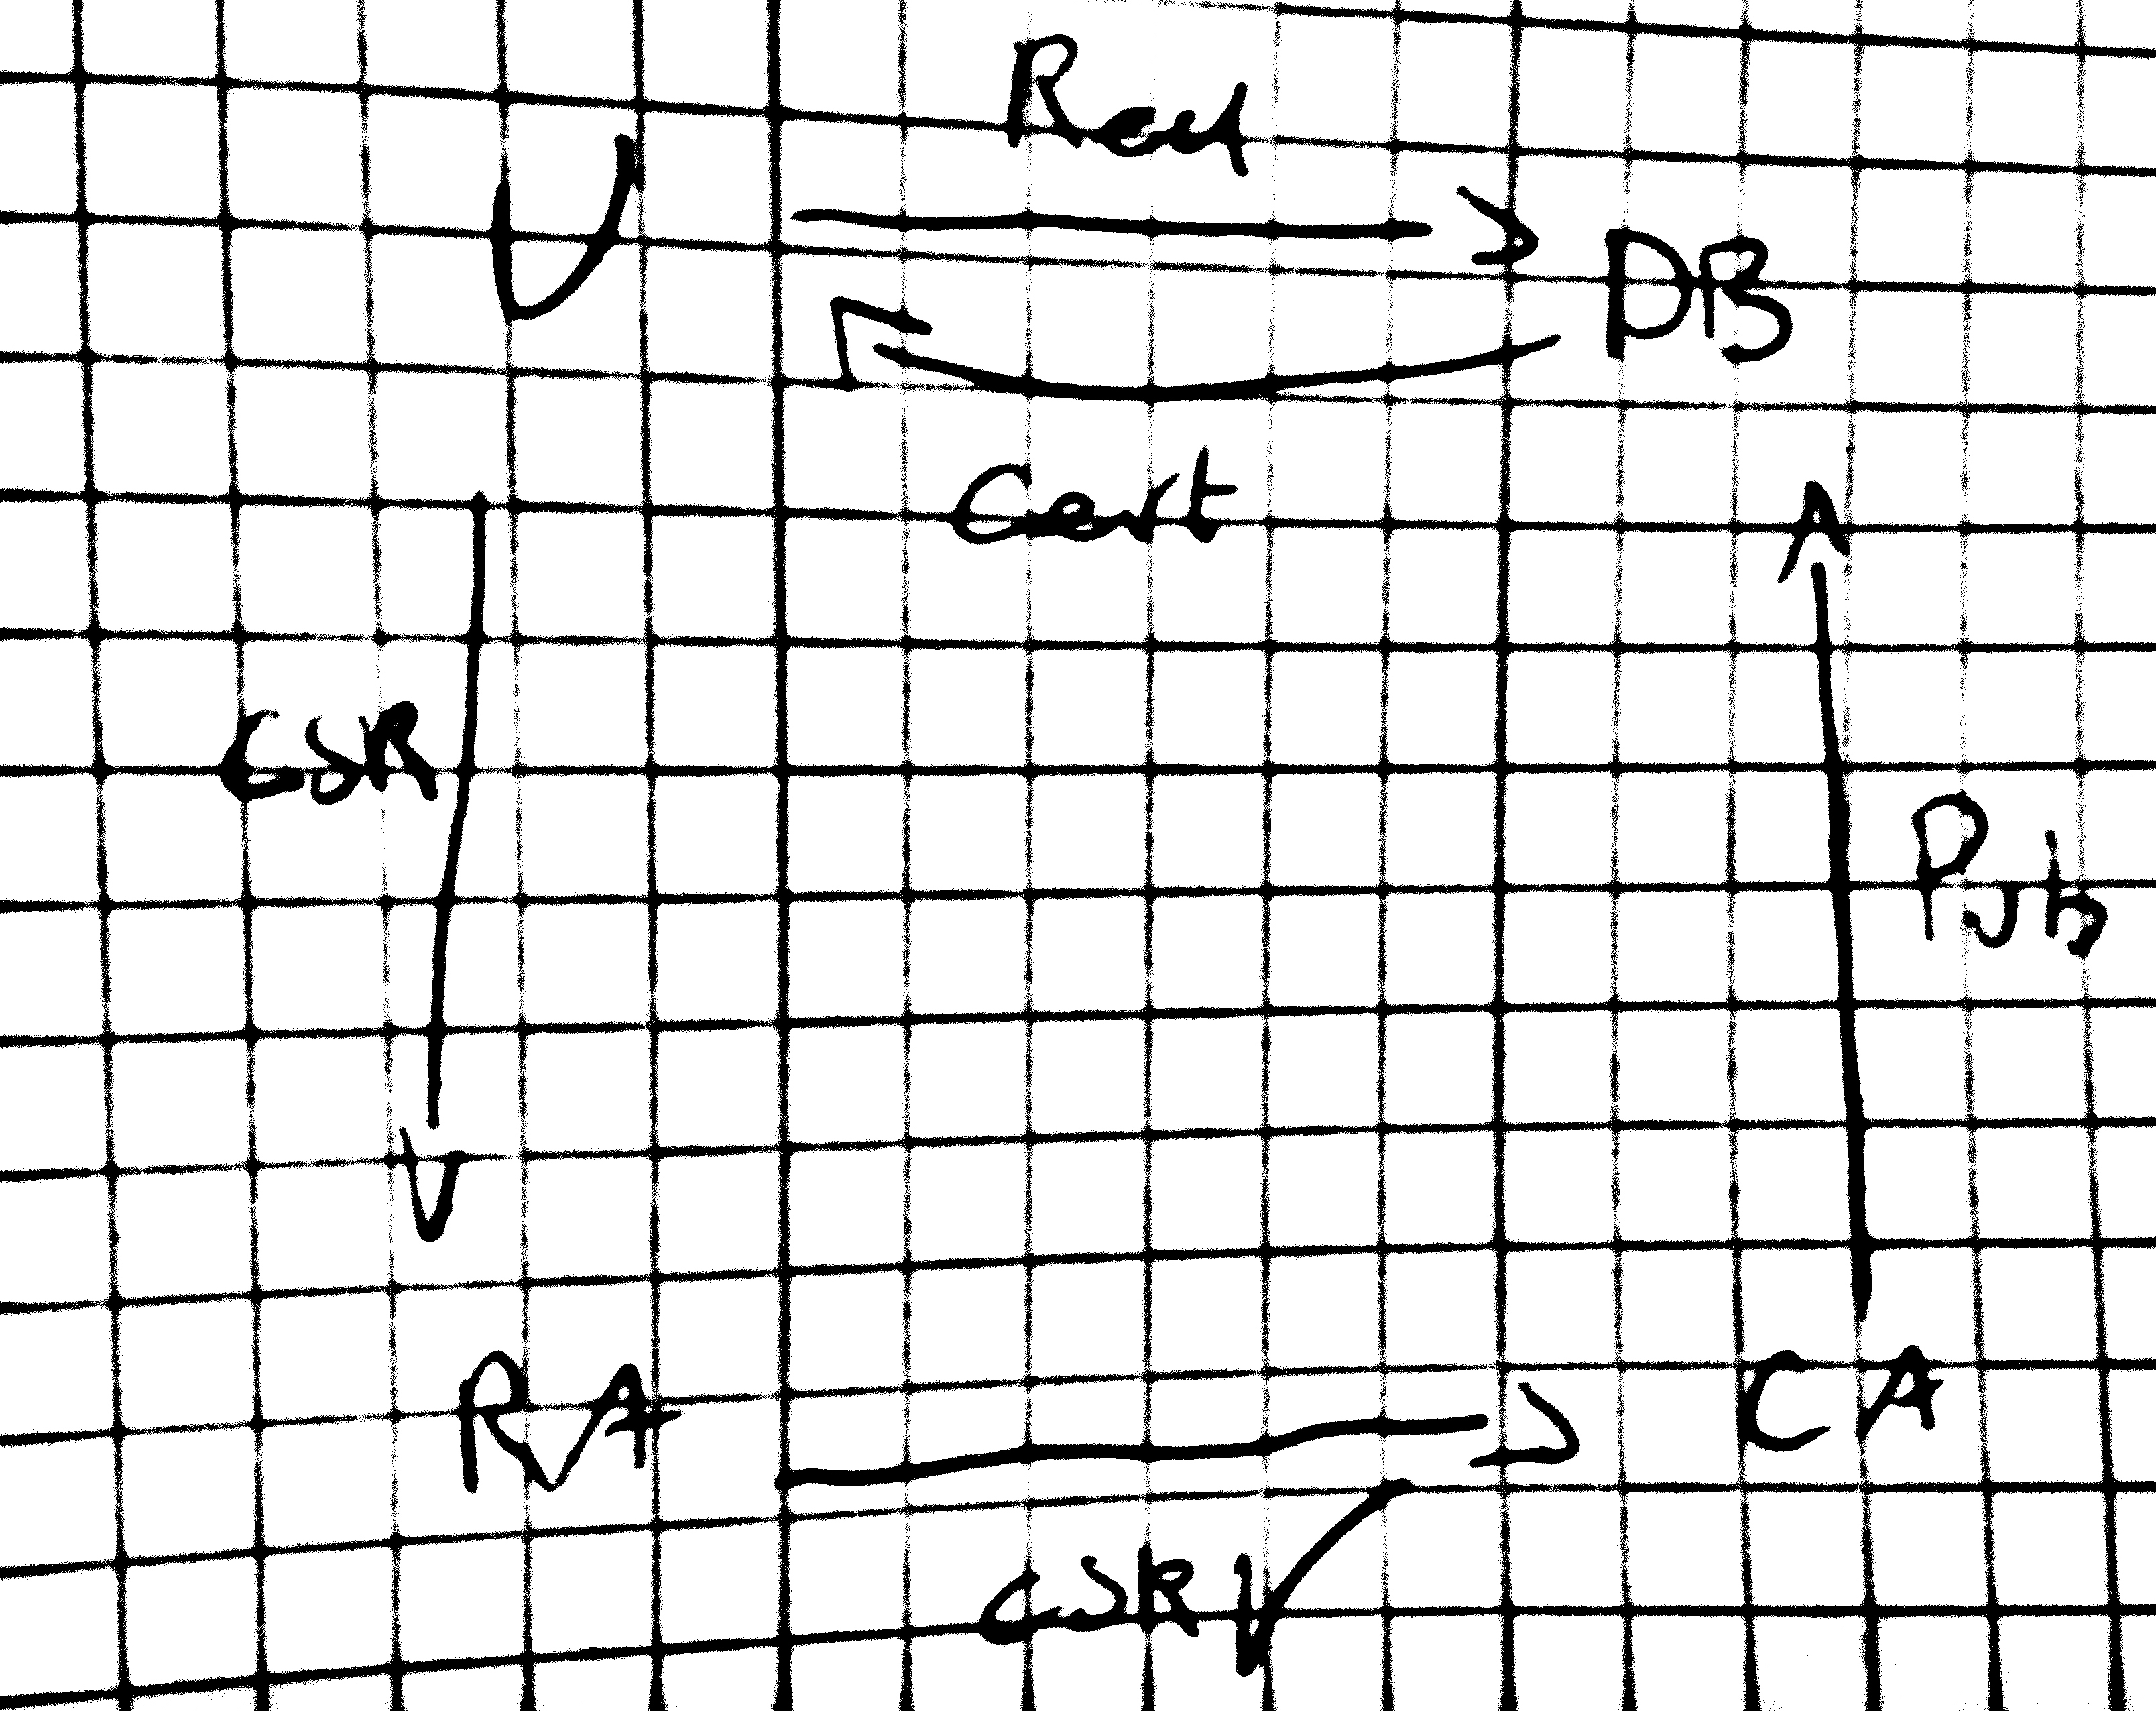
\includegraphics[width=0.6\textwidth]{pki}

\end{solution}
\part Si descrivano i modelli di rilascio dei certificati centralizzato e a tre parti servendosi di opportuni schemi.
\begin{solution}
Il modello centralizzato di rilascio di certificati prevede due sole parti: utenti e CA.
La CA genera le chiavi a seguito delle richieste e le invia agli utenti attraverso un canale sicuro.
In questo caso sono possibili due soluzioni:
	\begin{enumerate}
		\item L'utente finale genera la propria chiave pubblica e chiede conferma alla CA; la chiave privata rimane sempre in mano all'utente finale, ma esso deve disporre di un generatore di chiavi.
		\item le chiavi sono generate direttamente dalla CA, che memorizza la chiave pubblica e invia all'utente finale il certificato e la chiave privata; l'utente non deve eseguire operazioni se non richiedere il certificato e se perde la chiave privata può richiederla alla CA, ma non c'è supporto al non ripudio perché la CA conosce la chiave privata.
	\end{enumerate}
Il modello centralizzato viene utilizzato solo in situazioni nelle quali un'azienda desidera far proteggere ai dipendenti i propri dati, ma vuole fungere da CA per poter decrittare in caso di attacco di criptazione da parte di un dipendente malevolo.
Il modello a tre parti, invece, prevede tre entità: utenti, RA e CA.
In questo caso è possibile agire in tre modi:
\begin{enumerate}
\item Ogni utente si identifica di persona presso la RA, la quale invia le informazioni dell'utente alla CA che produce il certificato, crea una entry nella directory e inoltra il certificato alla RA che lo gira all'utente.
\item Ogni utente si identifica di persona presso la RA, la quale genera un segreto che l'utente potrà usare per ritirare le chiavi presso la CA, che le genera \textit{out of band}.
\item Ogni utente genera le chiavi e richiede un certificato alla CA, che inoltra la richiesta alla RA la quale la approva e la rimanda indietro, permettendo alla CA di produrre il certificato.
\end{enumerate}
Di seguito sono riportati gli schemi di funzionamento nei tre casi.

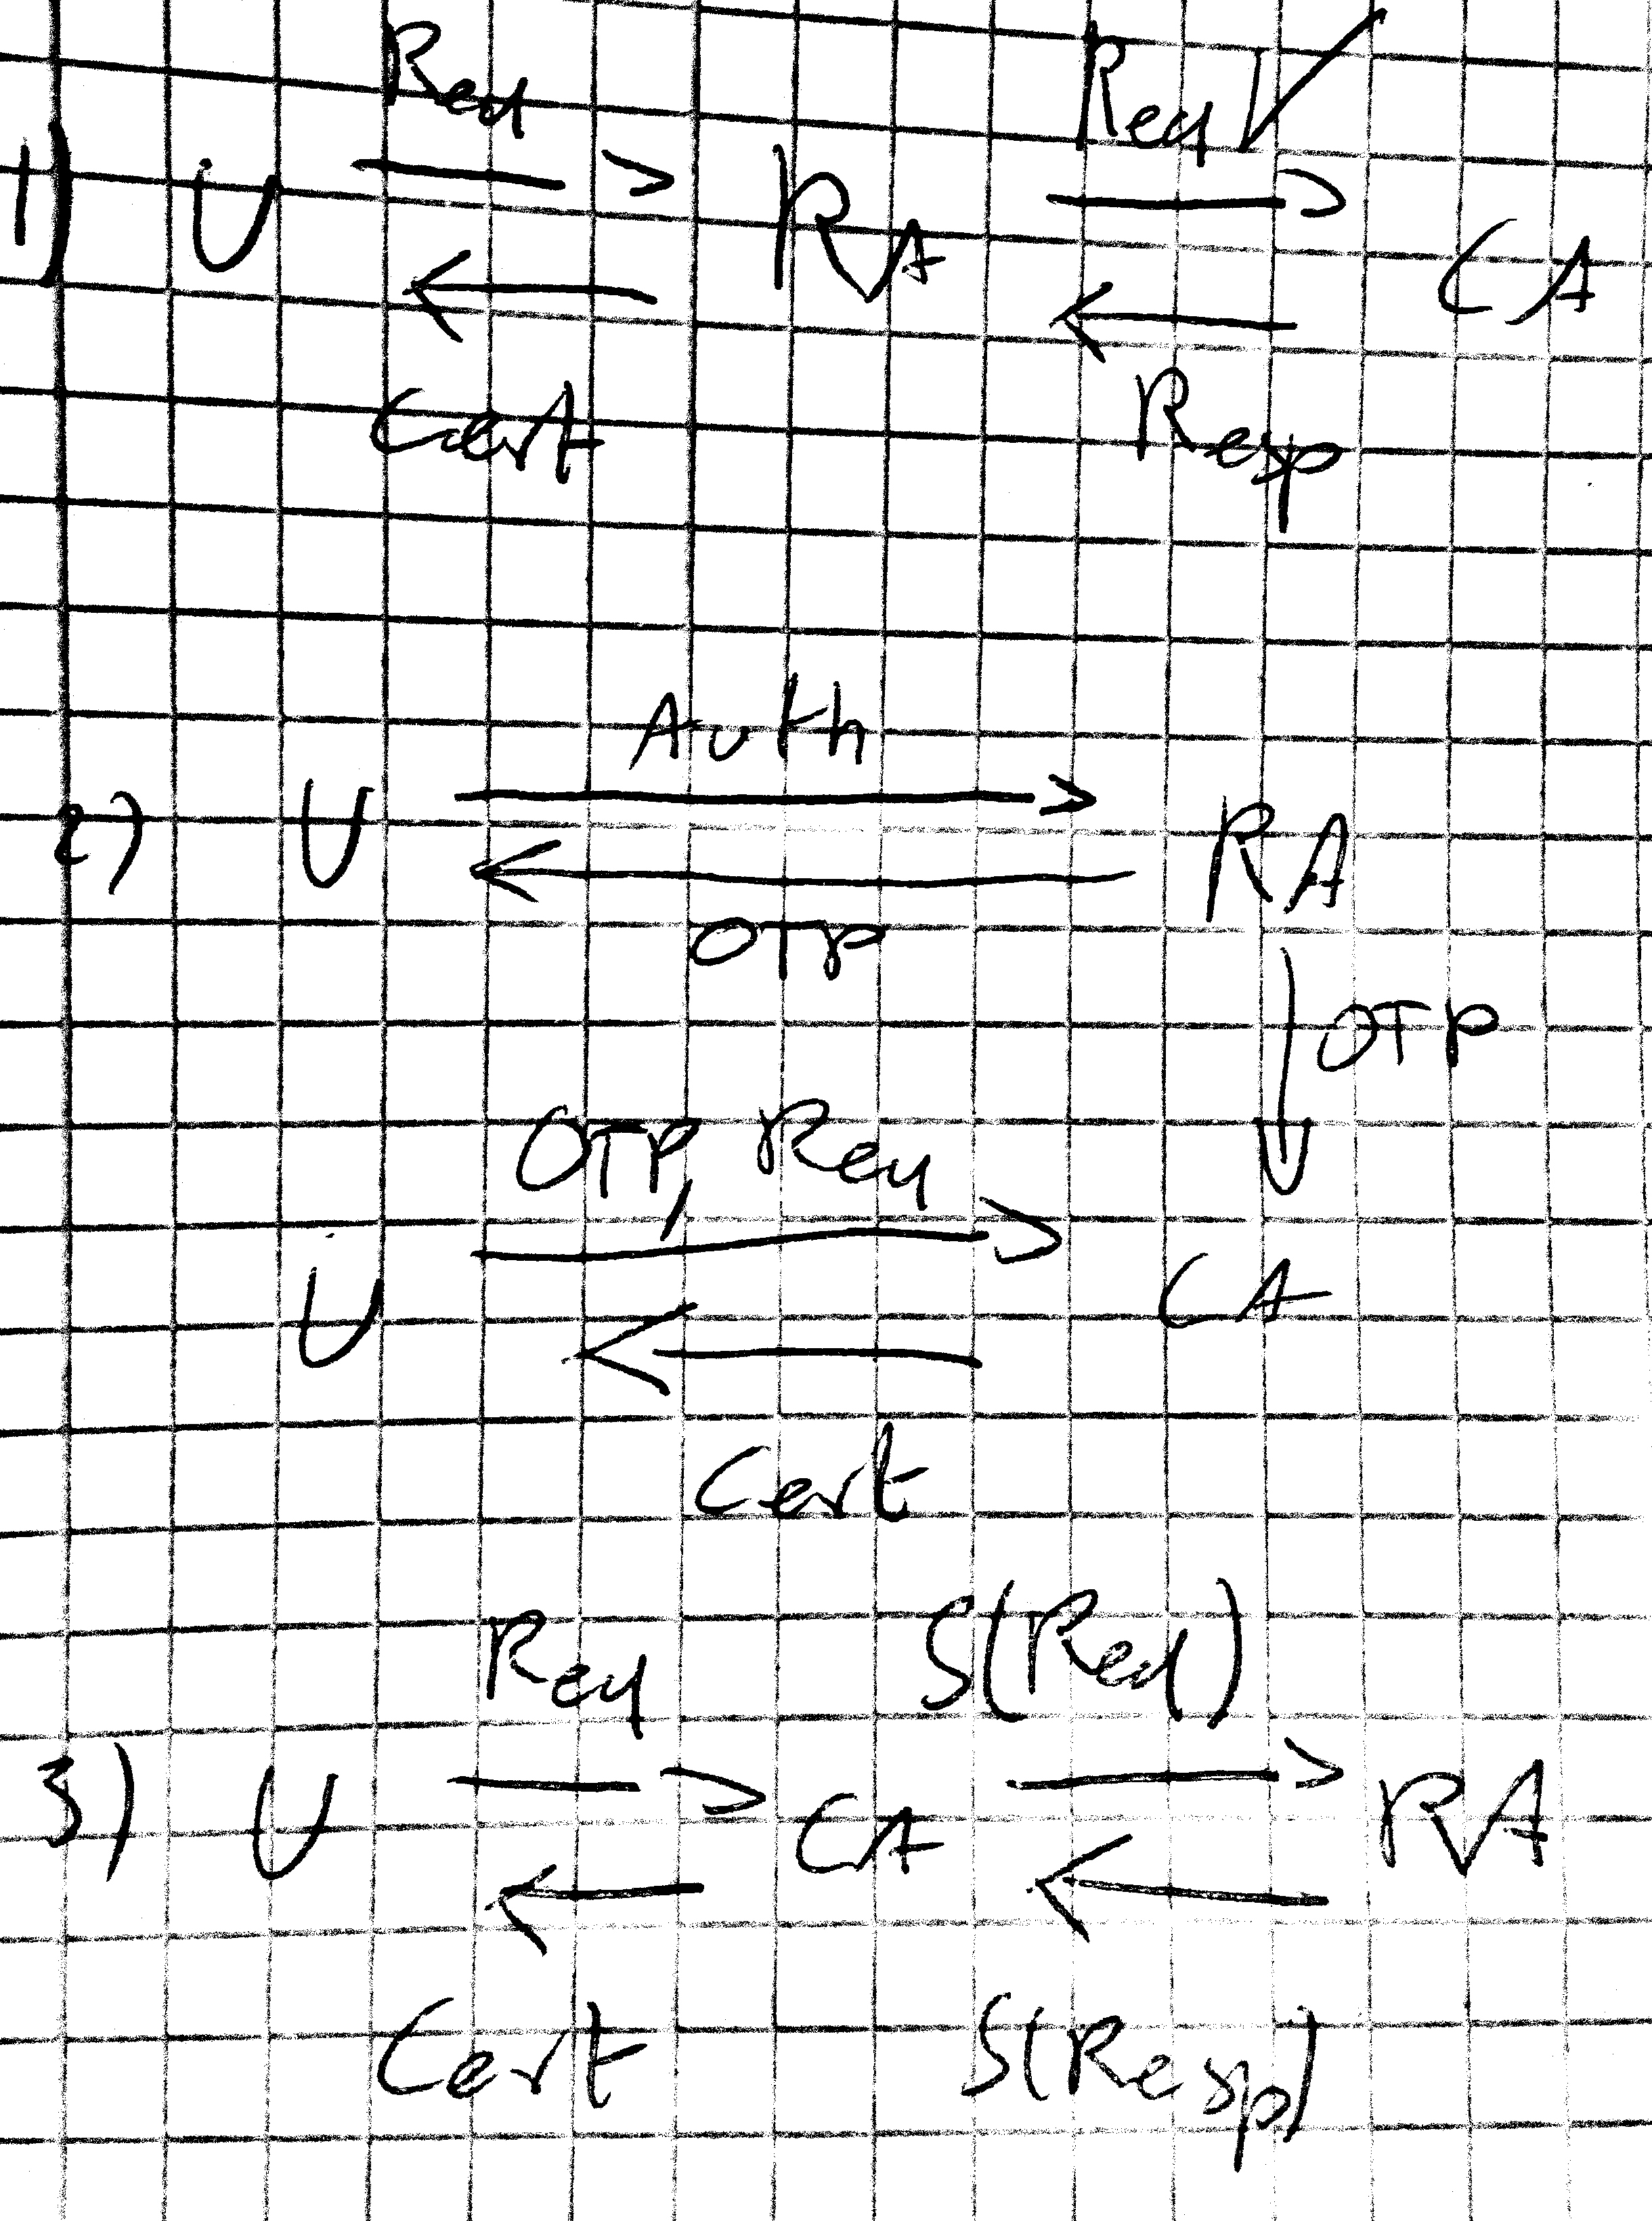
\includegraphics[width=0.6\textwidth]{certauth}

Il primo modo è costoso in quanto ogni utente deve possedere una smart card o dispositivo simile e presentarsi di persona, ma la CA non è esposta.
Il secondo modo espone la CA all'esterno, ma comunque meno del terzo modo che è per questo il meno utilizzato.
\end{solution}
\part Si tracci uno schema di richiesta presso RA con proof of possession (POP). Si descriva la certification path.
\begin{solution}
Per evitare che chiunque, impersonando un altro utente, richieda alla CA un certificato fornendo solo la chiave pubblica, la CA deve avere garanzie sul possesso della chiave privata da parte di chi richiede un certificato.
Un metodo di fornire la POP è formulare la richiesta come un messaggio cifrato e firmato digitalmente contenente il proprio ID e la propria chiave pubblica.
In questo modo, la CA può verificare la firma e, con essa, il possesso della chiave privata da parte del richiedente.
Questo metodo è il protocollo PKCS\#10.
Il metodo più sicuro sarebbe la POP a tempo di firma, ovvero l'inserimento in tutti i messaggi di un riferimento al certificato firmato con la propria chiave privata.
In questo modo, la destinazione può verificare la firma ed essere certo dell'identità del mittente.
Questo metodo, tuttavia, non è ancora supportato dai protocolli.
Esistono altri metodi online, come l'utilizzo di sfida e risposta o l'invio di un certificato cifrato che viene revocato in caso di inutilizzo, il quale lascia presupporre che il richiedente non fosse in possesso della chiave privata necessaria per decifrarlo.
Esistono inoltre metodi out-of-band in cui la RA o la CA generano le chiavi e le rilasciano personalmente tramite smart card o crypto token.
Tuttavia, questi metodi non garantiscono il non ripudio: chi genera i certificati mantiene una copia di tutte le chiavi private.
\end{solution}
\part Descrivere i meccanismi di revoca basati su CRL e sul protocollo OCSP evidenziandone anche le differenze principali.
\begin{solution}
La revoca di un certificato prima della sua scadenza diventa necessaria qualora, ad esempio, la chiave privata venga compromessa.
In questo caso, il ripudio della chiave, che comporta la revoca del certificato, deve essere comunicata tempestivamente alla RA e la CA deve comunicare a tutti gli utenti la revoca del certificato corrispondente.
In questo caso è possibile seguire un modello push, nel quale la CA comunica a tutti la revoca, o un modello pull, nel quale sono gli utenti a controllare le revoche su un database.
Un'ulteriore classificazione dei modelli di controllo delle revoche è la divisione tra modelli online e offline.
In generale si adottano solo modelli pull dato che un modello push richiederebbe un protocollo publisher/subscriber, molto complesso da gestire e poco scalabile, che viene utilizzato solamente se è necessario ricevere notifiche in tempo reale.
	Le Certificate Revocation List sono uno schema pull disponibile sia online che offline offline che prevede che la CA mantenga una lista autenticata dei certificati revocati, disponibile su una directory LDAP e che può essere scaricata e visionata offline.
Questa lista viene periodicamente aggiornata e contiene informazioni sul proprio periodo di validità.
Il problema principale di una CRL è la dimensione della stessa, che cresce con l'aggiunta di nuove revoche; inoltre, le CRL vengono rilasciate periodicamente e quindi non c'è freschezza delle informazioni.
	Il periodo di aggiornamento dipende dalla CA e la struttura dati è valida solo in un certo intervallo temporale.
È possibile risolvere il problema della grande dimensione eliminando i certificati già revocati a ogni nuova pubblicazione o dopo la loro scadenza, pubblicando aggiornamenti incrementali (Delta CRL) invece di ripubblicare l'intera lista costantemente, o partizionando la CRL in vari gruppi.
Eliminare le revoche già pubblicate o aggiornare la lista in maniera incrementale fa ricadere sull'utente l'onere di scaricare pubblicazioni passate fino a ricostruire l'intera lista.
La CRL viene partizionata secondo il numero seriale dei certificati.
	A questo punto, nel campo estensioni di ogni certificato viene specificato il valore del CRL Distribution Point (CRLDP), ovvero l'URL della partizione che conterrà una eventuale revoca.
	Il protocollo OCSP è un modello pull online che permette di disporre di informazioni sempre aggiornate provenienti direttamente dalla RA e non da liste offline.a
	La RA può verificacre al momento dellla richiesta se un certificato è valido o è stato revocato; lel risposte sono firmate dal servr OCSP e non dalla CA, che si limiterà a cetificare le chiavi del server.
	Chiaramente, il certificato del server non è verificabile con OCSP.
	I server OCSP possono non essere gli stessi che offrono anche le CRL.
	Sono possibili due architetture di OCSP: risposte pre-calcolate, che diminuiscono il carico del server e permettono al client di non dover scaricare tutta la CRL per ottenere un solo certificato, ma rendono possibili attacchi di replay; o attingere direttamenete dalla RA e non dalle CRL, meccanismo che però non è implementato dal protocollo OCSP.
Per questi motivi, l'utilizzo di OCSP è preferibile quando è necessaria freschezza delle informazioni e quando si vuole evitare di far gravare sull'utente l'onere di scaricare una struttura dati potenzialmente molto pesante.
	I responder OCSP si dividono in \textit{trusted} e \textit{delegated}.
	I trusted responder  firmano le risposte con una coppia di chiavi diversa e indipendente da quella della CA per cui sta rispondendo.
	In genere, i trusted responder sono aziendali o pagati dagli utenti.
	I delegated responder firmano  le risposte con una coppia di chiavi diversa in base allla CA per cui stanno rispondendo.
	In genere, i delegated responder sono pagati dalle CA.
\end{solution}
\part Com'è organizzato il sistema di directory X500 in cui sono poste le CRL?
\begin{solution}
Dato che il protocollo X.500 è molto costoso, viene utilizzata una versione più leggera chiamata LDAP.
Si tratta di un sistema di nomi gerarchico in cui ogni entry contiene una coppia tipo-valore.
La directory memorizza tutti i certificati relativi agli utenti e le informazioni sulla revoca dei certificati.
La directory deve essere sempre disponibile ed accessibile emolto scalabili.
	Seguendo lo standard X.500, la directotry è un sistema distribuito in cui ogni database è chiamato DSA (Directory Service Agent) e tutti gli utenti che vogliono accedervi utilizzano il DUA (Directory User Agent).
	I DSA sono distriubiti geograficamente e coordinare in modo tale da replicare l'informazione e assicurare scalabilità.
	Se un DSA non possiede in locale un certificato richiesto, essa lo chiederà ad altri DSA.
	L'accesso alle directory può essere o meno autenticato.
	Se si accede per scaricare la lista dei certificati non è necessaria l'autenticazione, perché il dato è pubblico.
	Le informazioni sono memorizzate come entry in un albero gerarchico.
	Ogni entry è associata a una classe oggetto che ne definisce le caratteristiche strutturali e, di conseguenza, gli attributi interni a ciascuna entry.
	Ogni attributo ha un tipo (classe utente, classe certificato ecc. ecc).
	Lo schema organizzativo della direcotry viene scelto nel momento dell'implementazione iniziale in base allo scopo della directory stessa.
	Ogni entry è identificata da un distinguish name (DN), un nome che indica il percorso assoluto, partendo dalla root, che identifica in maniera univoca una determinata entry, e da un relative distinguish name (RDN).
Per trovare un'entità in una CRL viene specificato solo il DN dell'entità menzionata nel certificato: le informazioni che contiene (azienda, Stato, dipartimento ecc.) sono una sequenza di RDN che vengono usati per trovare l'entità richiesta.
\end{solution}
\part Che cos'è una chain of trust? Si mostri un esempio di CA path discovery. Cos'è una Authority Revocation List?
\begin{solution}
Dato un grafo in cui i nodi sono CA e ogni arco indica che il nodo da cui parte ha fornito un certificato (detto cross-certificate) in favore del nodo a cui arriva, una chain of trust è un cammino che collega due CA.
Si rende necessaria la costruzione di una chain of trust quando due utenti che vogliono comunicare fanno riferimento a due CA diverse.
Un dominio di certificazione è costituito da tutti i rilasci di certificati che hanno come origine una data CA.
Ognuno dei due utenti deve attraversare più domini di certificazione fino a raggiungere quello dell'altro utente.
A ogni attraversamento di dominio di certificazione vanno verificati la firma digitale, il periodo di validità ed eventuali revoche del cross-certificate, oltre alle politiche di rilascio che non sono standardizzate e variano fra le CA.
Un esempio di CA path discovery è mostrato nello schema seguente.
Si noti che è possibile costruire una chain of trust dalla CA 0 alla CA 3, ma non il contrario.
Il grafo mostrato non è strutturato e corrisponde a un modello di fiducia distribuito.
Un altro modello di fiducia è quello gerarchico, nel quale il grafo è un albero.
Questo modello, però, richiede fiducia assoluta nella CA radice.
Se gli archi sono tutti unidirezionali, si parla di modello gerarchico top-down.
Ovviamente anche i certificati generati in favore di altre CA sono revocabili: in questo caso, invece che di CRL, si parla di ARL.

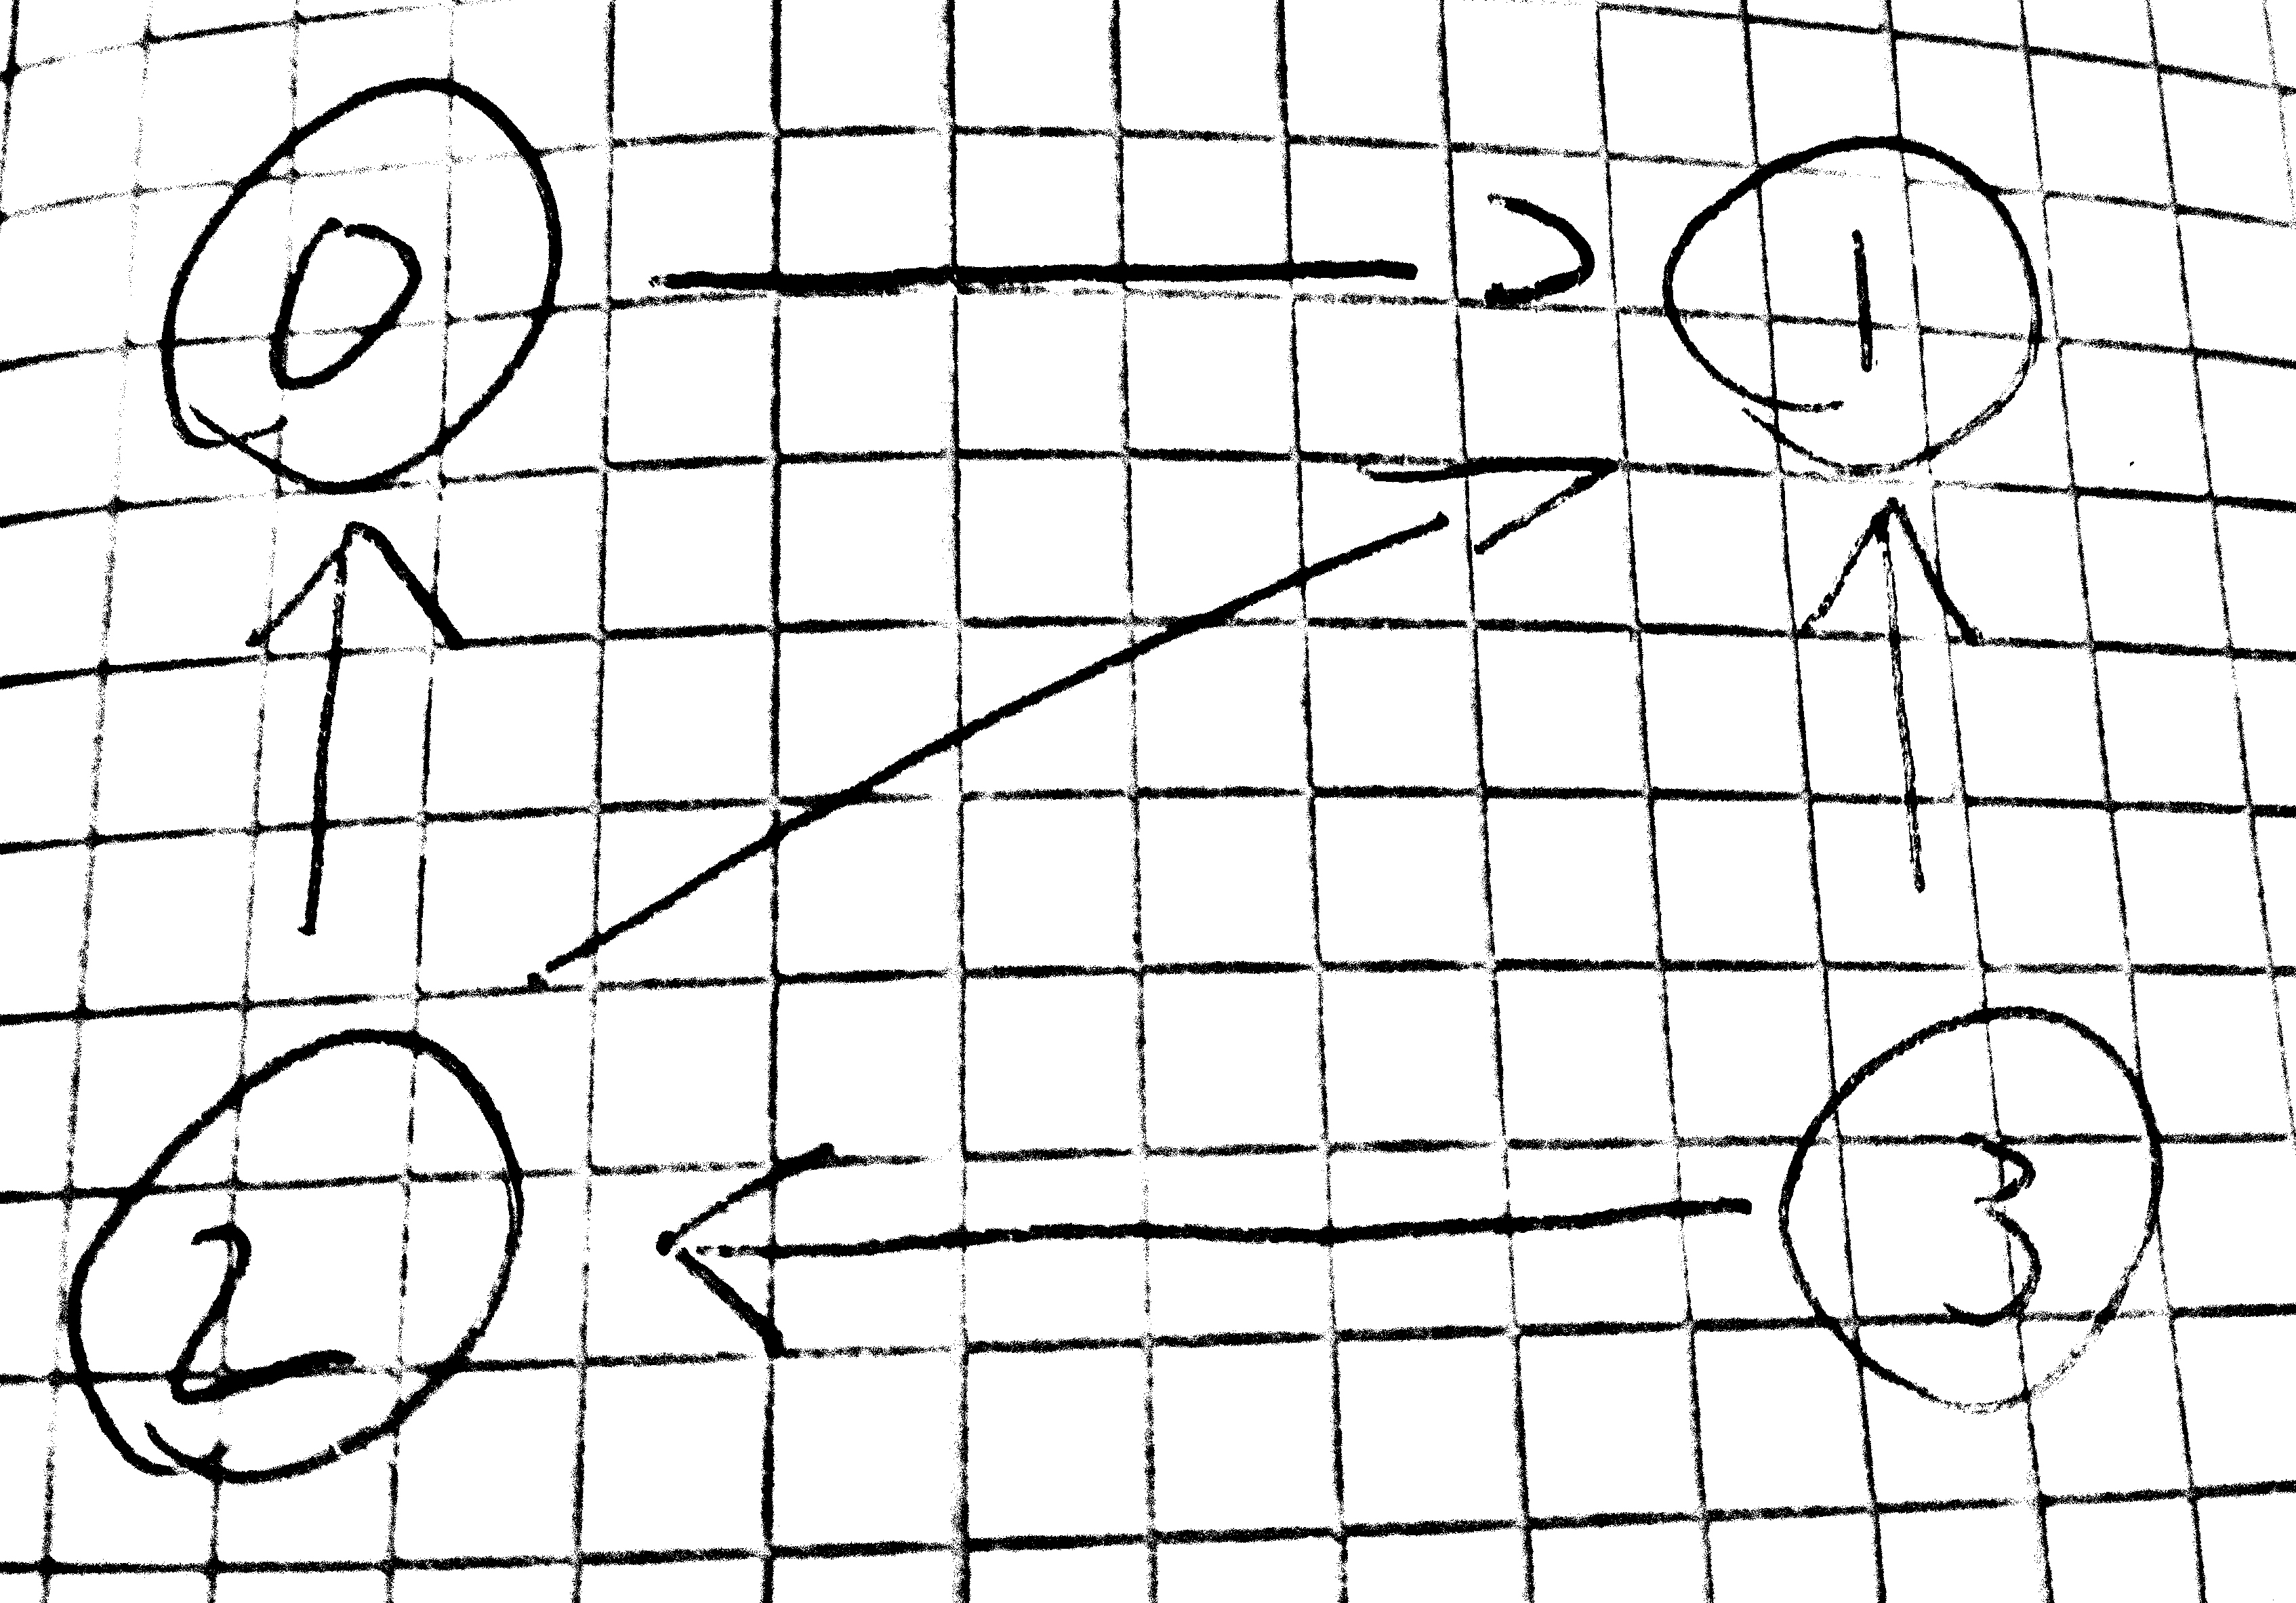
\includegraphics[width=0.6\textwidth]{capathdisc}

\end{solution}
\part Si descriva il funzionamento di PGP. Perché PGP genera la firma prima di applicare la compressione?
\begin{solution}
PGP è un programma di crittografia in grado di garantire autenticazione, integrità e confidenzialità.
PGP si serve di cifrari simmetrici con modalità CFB per la cifratura, cifrari asimmetrici (RSA o DH ElGamal) per la distribuzione di chiavi, e della firma digitale con appendice per l'autenticazione.
PGP non usa una CA ma si basa invece sulla costruzione di una rete di fiducia reciproca: per questo motivo la fiducia ha una componente soggettiva e PGP non ha valore legale.
Per generare le chiavi, PGP si avvale di un TRNG che genera continuamente dati casuali i quali vengono sottoposti a XOR e hashing prima di venire salvati in un archivio, detto random pool, dalla quale poi vengono estratti i bit necessari per generare le chiavi private e i seed del PRNG.
Il PRNG di PGP, usato per le chiavi di sessione e i vettori di inizializzazione, si basa sullo standard ANSI X9.17.
Ogni utente dispone di un portachiavi privato nel quale sono salvate le sue chiavi private, cifrate con un cifrario simmetrico che usa come chiave lo hash di una passphrase, e di un portachiavi pubblico nel quale vengono salvate le proprie chiavi pubbliche e quelle dei corrispondenti.
Per firmare e cifrare un messaggio con PGP, la sorgente:
\begin{enumerate}
\item estrae dal proprio portachiavi privato una chiave di firma $S_A$ e la decifra utilizzando il cifrario simmetrico $D_k(\cdot)$ in cui la chiave è lo hash della passphrase;
\item firma $H(m\concat t)$ con la propria chiave di firma;
\item estrae dal proprio portachiavi pubblico la chiave di cifratura $P_B$ della destinazione;
\item genera la chiave di sessione $k$ servendosi del proprio random pool;
\item cifra $k$ concatenato con il nome del cifrario simmetrico e un checksum del messaggio;
\item cifra il messaggio firmato mediante il cifrario simmetrico $E_k(\cdot)$;
\item invia alla destinazione il messaggio firmato con la propria chiave e cifrato con $E_k(\cdot)$ concatenato con la chiave pubblica e il checksum cifrati con la chiave $P_B$, il tutto concatenato all'ID della chiave della destinazione.
\end{enumerate}
Per decifrare questo messaggio, la destinazione mette in chiaro la propria chiave privata, decifra la chiave di sessione, la utilizza per decifrare il messaggio, estrae la chiave pubblica della sorgente dal proprio portachiavi, mette in chiaro lo hash del documento e verifica che l'impronta corrisponda.
Per permettere la trasmissione di un messaggio cifrato tramite e-mail ci si serve della trasformazione base64: il messaggio vene scomposto in blocchi da 24 bit, a loro volta divisi in 4 stringhe di 6 bit, e ogni stringa viene poi sostituita al byte che, in ASCII 8-bit, rappresenta il carattere (stampabile) a cui corrisponde.
Lo schema di autenticazione di PGP appone la firma prima della compressione per evitare che, firmando il messaggio compresso, la destinazione debba mantenere memorizzati sia il messaggio che la sua versione compressa per verificarne l'autenticità.
Inoltre, il compresso può essere sempre diverso.
Lo schema di riservatezza di PGP, invece, comprime e poi cifra, per eliminare eventuali ridondanze nel testo e renderlo più sicuro.
\end{solution}
\end{parts}
%PKI e PGP.
\question \textbf{Protocolli per la comunicazione sicura. Sicurezza a livello di rete: IPSEC, VPN. Sicurezza a livello di trasporto: SSL/TLS.}
\begin{parts}
\part Si descriva SSL/TLS. Come funziona? Quali protocolli se ne servono? Cosa garantisce?
\begin{solution}
SSL/TLS è una suite di 4 protocolli di sicurezza a livello di trasporto, progettati per essere collocato tra HTTP e TCP, in grado di garantire confidenzialità, autenticazione e integrità dei messaggi scambiati su una socket TCP.
SSL/TLS garantisce semitrasparenza per le applicazioni: non è l'applicazione a dover garantire la confidenzialità prima di inviare il dato su una socket, se ne occupa SSL/TLS.
SSL/TLS viene usato, tra gli altri, dal protocollo HTTPS.
SSL/TLS è strutturato in più protocolli: handshake, change cipherspec, alert, record.
	\begin{itemize}
		\item Handshake si occupa di negoziare tra client e server i meccanismi di sicurezza, cosa che si rende necessaria dato che non è sempre possibile sapere in anticipo quali siano supportati da entrambe le parti, e le chiavi da utilizzare. È un protocollo a livello applicativo che definsice una sessione, all'interno della quale vengono create più connessioni 
		\item Change cipherspec si occupa di rinegoziare, se necessario, i parametri e i meccanismi della connessione. È un rpotocollo a livello applicativo.
		\item Alert si occupa di gestire eventuali segnalazioni di allarme. È un protocollo a livello applicativo. 
		\item Record  si occupa effettivamente di calcolare e verificare le firme e di cifrare e decifrare i dati. È un protocollo a livello di trasporto che realizza il concetto di sessione e connessione.  
	\end{itemize}
Il protocollo record realizza il concetto di sessione e connessione: il protocollo di handshake definisce una sessione, all'interno della quale vengono create più connessioni che utilizzano gli stessi parametri crittografici.
La cifratura avviene in maniera simmetrica, mentre autenticazione e integrità sono garantite da HMAC.
Lo stato di una sessione è definito da un ID, dal certificato X.509 del server, dai metodi di compressione, hashing e cifratura, e dal master secret che verrà usato per produrre le chiavi di sessione. 
Lo stato di una connessione, invece, è definito da due nonce $R_C, R_S$, due segreti utilizzati per il MAC delle due parti, due chiavi condivise per la cifratura dei dati delle due parti, un vettore di inizializzazione se si usa CBC e un numero di sequenza per ogni  messaggio scambiato.
In trasmissione il messaggio viene frammentato e se necessario compresso.
Poi, secondo le ddecisioni prese durante handshake, può essere utenticato o meno servendosi di HMAC e viene infine cifrato.
Al termine dellle elaborazioni il pacchetto è completato con un'intestazione.
In ricezione una volta eliminata l'intestazione viene operata prima la decifrazione, poi la verifica dell'autenticità e infine decompressione e ricomposizione.
L'ordine di ricezione è più oneroso, perché se il messaggio non è integro va comunque prima decifrato.
SSL non integra la gestione della revoca né viene garantito che il certificato provenga dall'URL che si sta visitando.
Si rende quindi necessario un controllo a livello di browser.
	Le prime versionid i SSL/TLS non garantivano \textit{perfect forward secrecy} perché tutte le comunicazioni venivano memorizzate in RAM, rendendo possibile intercettare la chiave grazie all'osservazioni delle sessioni precedenti.

			Il protocollo handshake è diviso in quattro fasi: accordo sugli algoritmi, autenticazione server e client, controllo dello scambio.
L'autenticazione del client presso il server è opzionale; il certificato server invece è obbligatorio sempre, a meno che non si stia usando DH anonimo.
Il client indica i meccanismi di sicurezza e di compressione di cui è dotato con un messaggio detto \textit{client hello} a cui il server risponde con un \textit{server hello} che contiene i meccanismi scelti.
Il client hello contiene anche un nonce $R_C$ e un ID di sessione, usato per distinguere tra i casi in cui è necessario creare una nuova sessione o fare riferimento a una già avviata.
In seguito, il server si autentica inviando il suo certificato X.509, eventualmente il parametro pubblico $Y_S$ per lo scambio DH, una \textit{certificate request} se anche il client si deve autenticare, e un segnale conclusivo di \textit{server hello done}.
	Il client risponde poi, se gli è stato richiesto, con un certificato, con il suo parametro $Y_C$ per lo scambio DH, ed eventualmente con una notifica di \textit{certificate verify} se desidera verificare con una sfida e risposta che il server possieda effettivamente la chiave privata corrispondente a quella pubblica fornita; al termine di questa fase si è concordato il \textit{master secret}, ovvero la chiave che si userà per cifrare i dati.
Infine, il protocollo change si serve di funzioni hash per controllare l'integrità dei dati scambiati.
	Gli hash sono inviati cifrati per assicurarsi che il segreto sia stato effettivamente concordato.

			Il protocollo change cipher spec viene eventualmente utilizzato per modificare le specifiche concordate, e la negoziazione viene conclusa con un messaggio \textit{finished}.
Al termine dello handshake inizia il protocollo record per scambiare in maniera sicura dati.
SSL non supporta il non ripudio perché usa segreti condivisi dedotti dal master secret durante lo handshake.
\end{solution}
\part Quali meccanismi di scambio di chiavi possono essere usati con SSL/TLS?
\begin{solution}
È possibile servirsi degli schemi DH anonymous, fixed o ephemeral oppure scambiare le chiavi con RSA (servendosi quindi di un cifrario ibrido).
Non avrebbe senso utilizzare un KDC perché poco scalabile, né una master key dato che le chiavi non sono precondivise.
Se si usa DH anonymous, sorgente e destinazione definiscono i parametri $p, g$ all'inizio della sessione e a ogni connessione si scambiano due nonce $R_C, R_S$, in modo da prevenire gli attacchi replay e rendere casuale la chiave per ogni connessione senza dover ripetere l'intero scambio DH.
I segreti usati in cifratura ed autenticazione dei dati sono ottenuti a partire dal master secret condiviso
all’inizio della sessione.
Se si usa DH fixed, le due parti si scambiano $p, g$ all'interno di un certificato ricevuto da una CA che contiene anche $Y_C, Y_S$: diventa ancora più importante la presenza dei nonce, dato che il certificato rimane fisso per tutta la sessione.
Se si usa DH ephemeral, le due parti dispongono di una chiave pubblica certificata e di una chiave privata che utilizzano per firmare i parametri $Y_C, Y_S$ che vengono generati all'inizio di ogni connessione.
Con questo metodo l'uso dei nonce non è necessario, ma la loro presenza è comunque assicurata per motivi di uniformità.
	Nel caso generale  DH ephemeral non mi garantisce l’autenticazione del server. In SSL, però, tramite il protocollo di negoziazione si riesce a garantire anche l’autenticazione: è quindi leggermente diverso lo schema, perché prevede che la firma apposta dal server sia fatta anche sui parametri Rc e Rs scambiati all’inizio della sessione, nel messaggio \textit{server\_hello}.
Se si usa un cifrario ibrido, solo il client sceglie la chiave di sessione e la comunica al server criptandola con RSA, servendosi di una chiave pubblica estratta dal certificato che il server ha inviato al client.
\end{solution}
\part Si confrontino le modalità di garanzia di sicurezza di SSL/TLS e IPSec. Cosa viene garantito dai due protocolli in termini di riservatezza e autenticazione?
\begin{solution}
SSL/TLS è un protocollo di sicurezza a livello di trasporto, mentre IPSec è implementato a livello di rete.
IPSec può proteggere tutto il traffico scambiato tra due nodi, anche se le applicazioni al livello superiore non implementano sistemi di protezione.
SSL/TLS, invece, può proteggere il traffico scambiato a livello di singola applicazione.
SSL/TLS garantisce l'autenticazione delle parti e l'origine dei dati servendosi di algoritmi di firma digitale.
IPSec garantisce la riservatezza dei pacchetti in caso di intercettazione, certifica l'origine deii dati (proteggendo da spoofing e hijacking) servendosi di cifrari simmetrici o firma digitale e protegge da attacchi di Denial of Service.
Nel caso di SSL, la riservatezza è sempre garantita, mentre in IPSec questa granzia è opzionale.
In entrambi i casi la riservatezza, se richiesta o prevista dal protocollo, è garantita usando cifrari simmetrici.
\end{solution}
\part Si descrivano IPSec, SA, SAD e SPD e si illustri il flusso dei pacchetti.
\begin{solution}
IPSec è un'architettura che permette di rendere sicura la comunicazione mediante il protocollo IP.
Essa prevede tre componenti architetturali: Security Association, Security Association Database e Security Policy Database.
	\begin{itemize}
		\item 	Una SA è una struttura dati che identifica una connessione e i servizi di sicurezza utilizzati per essa.
Una SA è identificata da tre parametri: un Security Parameters Index, un IP di destinazione e il protocollo utilizzato (AH o ESP).
Il SPI permette alla destinazione di trovare la SA giusta per decodificare il pacchetto: viene concordata tra sorgente e destinazione e inviata insieme al pacchetto IPSec.
Le SA non sono fisse, ma vengono generate e personalizzate per le varie connessioni.
Per avere una protezione completa di un canale bidirezionale occorrono due connessioni logiche unidirezionali. 
\item Il SAD tiene traccia di quali tipi di servizi siano stati serviti, in che modo e dove siano indirizzati i pacchetti coinvolti, associando una SA a ogni servizio.
In questo modo è possibile determinare quali algoritmi vadano applicati per proteggere un pacchetto IPSec e per decodificarlo una volta ricevuto.
Il SAD contiene i parametri di ogni SA: il suo tempo di vita, le informazioni necessarie per AH/ESP, la modalità usata (tunnel o transport).
Ogni host o gateway IPSec ha il proprio SAD.
\item Il SPD invece esamina tutto il traffico IP in ingresso e in uscita e decide quali pacchetti abbiano bisogno di quali servizi e politiche IPSec.
	Ciascuna politica contenuta specifica una porzione di traffico IP e la SA da usare per quella porzione. 
			Una porzione di traffico è specificata tramite un insieme di selettori: IP di sorgente/dest, user ID, protocollo ecc ecc. 
			Si può anche richiedere la \textit{non protezione} di una comunicazione. 
	\end{itemize}
Per inviare un messaggio, si interroga il SPD per decidere le regole da applicare in base ai contenuti del messaggio stesso.
In seguito viene creata una nuova SA e inserita nel SAD, o letta una esistente, vengono applicati gli algoritmi richiesti dalla SAD e il pacchetto così creato viene trasmesso.a

	Il comportamento è speculare in ricezione: la SA appropriati viene cercata nel SAD in base al SPI (Security Parameters Index), si applicano gli algoritmi relativi, viene verificato mediante la policy estratta dall'SPD se il pacchetto sia stato protetto adeguatamente e si arriva infine al pacchetto IP originario.
\end{solution}
\part Si descrivano IPSec tunnel e transport. Come viene creato un pacchetto IPSec nelle due modalità? Quando è più opportuno usare l'uno o l'altro?
\begin{solution}
Nella modalità IPSec transport il pacchetto creato conserva invariata l'intestazione del pacchetto originale, che contiene gli indirizzi IP di sorgente e destinazione.
Questa modalità può essere sicuramente applicata in tutte le possibili configurazioni di IPSec.
Cio è vero perché non alterando l'intestazione, il pacchetto IPSec risultante è sempre instradabile.
Si ricordi che IPSec può essere applicato tra due end system, due gateway o un end system o un gateway.
La modalità tunnel si chiama così perché tutto il pacchetto viene incapsulato all'interno di un nuovo pacchetto IPSec che a differenza di quello originale contiene potenzialmente un indirizzo IP destinazione diverso da quello del pacchetto oirignale.
Dall momento che  questo pacchetto IPSec ha nuovi indirizzi di sorgente e destinazione, non si può comunicare in modalità tunnel tra due end system, ma solo nel caso in cui il nodo finale voglia inviare un pacchetto IP a un nodo di una rete interna di cui non vuole far conoscere l'indirizzo IP: incapsula il proprio pacchetto all'interno di un  pacchetto IPSec nuovo in cui l'IP destinazione è quello del gateway, che riceve il pacchetto, lo ritrasforma in pacchetto IP e lo trasmette alla destinazione.
La modalità tunnel può essere utilzizata anche tra due gateway per proteggere tutte le comunicazioni tra due nodi senza far conoscere sorgente e destinazione: l'indirizzo IP sorgente diventa quello del gateway di partenza, quello della destinazione quello del gateway di arrivo.
\end{solution}
\part Si descrivano IPSec AH, ESP ed ESP con autenticazione. Che ordine seguono le operazioni di autenticazione e cifratura? Che differenze ci sono in ricezione tra SSL/TLS e IPSec e perché IPSec è più performante?
\begin{solution}
	L'Authentication Header è un protocollo per fornire un controllo di integrità, autenticità e protezione contror gli attacchi di replay. 
	Per l'autenticaizone crea uno hash con HMAC del pacchetto IP sfruttando un segreto condiviso.
	In modalità transport l'AH autentica il payload e porzioni dello header IP e degli extension header IPv6, tra cui l'IP del mittente, garantendo quindi protezione da IP spoofing. 
	In modalità tunnel l'AH autentica l'intero pacchetto interno, ma anche porzioni selezionate del pacchetto esterno; anche qui garantisce protezione da IP spoofing. 
L'Encrypted Security Payload è uno header apposto a un pacchetto di dati IPSec che la sorgente ha cifrato. 
L'uso di una chiave segreta concordata garantisce l'origine, la cifratura garantisce riservatezza.
IPSec ESP con autenticazione prevede che venga controllata l'integrità di un pacchetto mediante il campo Authentication Data, con il valore Integrity Check Value; se il pacchetto non proviene dal giusto destinatario, il pacchetto verrà decifrato male e fallirà il controllo ICV. 
IPSec prevede che in ricezione vengano verificate l'integrità e l'origine del pacchetto prima di procedere con la decifratura.
In caso di fallimento della verifica di integrità e origine, il pacchetto viene scartato senza essere decifrato.
Un messaggio inviato con SSL/TLS invece viene firmato prima di essere cifrato: al momento della ricezione, quindi, deve prima essere decifrato, ma se in seguito il controllo di integrità fallisce si è effettuata inutilmente un'operazione di decifratura.
\end{solution}
\part Si descriva il sub-protocollo anti-replay di IPSec. Si descriva il funzionamento della finestra a scorrimento.
\begin{solution}
IPSec realizza il proprio servizio anti-replay servendosi di un Sequence Number Field posseduto da ogni pacchetto.
Dato che IP non garantisce l'arrivo in ordine dei pacchetti, ci si serve di una finestra scorrevole per permettere di individuare comunque eventuali pacchetti duplicati.
Ogni volta che viene ricevuto un pacchetto, dopo averne verificato l'integrità, se il suo SNF è minore dell'estremo sinistro della finestra esso viene scartato.
Se il SNF si trova all'interno della finestra, invece, la casella corrispondente viene segnata come occupata, e se viene ricevuto un pacchetto con lo stesso SNF quest'ultimo viene scartato.
Se il SNF è maggiore dell'estremo destro della sequenza, invece, la finestra stessa viene spostata in modo che la casellla più a destra corrisponda con il SNF ricevuto.
Di default, la finestra è lunga 64 pacchetti.
\end{solution}
\end{parts}
\end{questions}
\section*{Notazione}
\begin{itemize}
\item $\concat$: operatore di concatenazione
\item $H(\cdot)$: funzione hash
\item $E, D$: funzioni di cifratura/decifratura (e.g. con un cifrario)
\item $S(\cdot)$: funzione di firma digitale
\item $V(\cdot)$: funzione di verifica firma
\item $t$: timestamp
\end{itemize}
\textbf{Disclaimer}:  Questo documento può contenere errori e imprecisioni che potrebbero danneggiare sistemi informatici, terminare relazioni e rapporti di lavoro, liberare le vesciche dei gatti sulla moquette e causare un conflitto termonucleare globale.
Procedere con cautela.
Questo documento è rilasciato sotto licenza CC-BY-SA 4.0. \ccbysa
\end{document}

